\documentclass[11pt]{article}
\usepackage[T1]{fontenc}
\usepackage{lmodern}
\usepackage{amsmath,amsthm,amssymb,mathtools}
\usepackage[margin=1.05in]{geometry}
\usepackage{microtype}
\usepackage{xcolor,enumitem,booktabs}
\usepackage{tikz}
\usetikzlibrary{arrows.meta,positioning}
\definecolor{linkblue}{rgb}{0.05,0.16,0.42}
\usepackage[colorlinks=true,linkcolor=linkblue,citecolor=linkblue,urlcolor=linkblue]{hyperref}
\usepackage[capitalise,noabbrev]{cleveref}
\hypersetup{pdftitle={Randomized quasipolynomial-time mean-payoff games},pdfauthor={OpenAI}}
\pdftrailerid{}
\setlength{\emergencystretch}{1.5em}
\clubpenalty=10000
\widowpenalty=10000
\displaywidowpenalty=10000
\setlist[enumerate]{itemsep=.4em,topsep=.5em}
\setlist[itemize]{itemsep=.25em,topsep=.4em}
\numberwithin{equation}{section}
\theoremstyle{plain}
\newtheorem{theorem}{Theorem}[section]
\newtheorem{lemma}[theorem]{Lemma}
\newtheorem{proposition}[theorem]{Proposition}
\newtheorem{corollary}[theorem]{Corollary}
\theoremstyle{definition}
\newtheorem{definition}[theorem]{Definition}
\newtheorem{procedure}[theorem]{Procedure}
\theoremstyle{remark}
\newtheorem{remark}[theorem]{Remark}
\crefname{procedure}{Procedure}{Procedures}
\Crefname{procedure}{Procedure}{Procedures}
\newcommand{\R}{\mathbb R}
\newcommand{\N}{\mathbb N}
\newcommand{\Z}{\mathbb Z}
\DeclareMathOperator{\Prb}{Pr}
\DeclareMathOperator{\clip}{clip}
\DeclareMathOperator{\supp}{supp}
\DeclarePairedDelimiter{\floor}{\lfloor}{\rfloor}
\DeclarePairedDelimiter{\ceil}{\lceil}{\rceil}
\newcommand{\Solve}{\ensuremath{\mathsf{Solve}}}
\newcommand{\Ask}{\ensuremath{\mathsf{Ask}}}
\newcommand{\Orient}{\ensuremath{\mathsf{Orient}}}
\newcommand{\OrientPlus}{\ensuremath{\mathsf{OrientPlus}}}
\newcommand{\Basic}{\ensuremath{\mathsf{Basic}}}

\title{Randomized quasipolynomial-time mean-payoff games}
\author{OpenAI}
\date{September 25, 2026}
\begin{document}
\maketitle
\begin{abstract}
We give a randomized algorithm that computes the complete zero-threshold
winning set of a finite mean-payoff game with arbitrary signed integer edge
weights encoded in binary. For total explicit input length $L$, it uses
$2^{O((\log(L+2))^2)}$ bit operations on every random tape and is correct
with probability at least $7/8$. A polynomial-time check certifies the winning
regions and positional strategies for both players or reports failure.
Independent repetition therefore gives an always-correct algorithm with the
same expected quasipolynomial bit bound.
\end{abstract}
\setcounter{tocdepth}{1}
\hypersetup{bookmarksdepth=2}
\tableofcontents
\clearpage
\section{Introduction}

A mean-payoff game asks whether a player can maintain a nonnegative
long-run average reward while an opponent chooses some of the moves.
The arena is finite, but plays are infinite and integer edge weights may
have large magnitudes. Positional strategies provide finite certificates
for the two winning regions. The algorithmic difficulty is to find those
regions with a cost controlled by the binary description, rather than by
the numerical size of a weight.

This paper gives a randomized quasipolynomial-time algorithm. Its central
output is an exact bounded integer potential: with probability at least
$7/8$, every coordinate of that potential is correct. Thresholding it
returns the complete winning set. The method also gives order guarantees
in finite integer boxes with arbitrary endpoints and the allowed reference
width. Each guarantee concerns a fixed comparison vector and all its
coordinates at once.

\subsection{Games, encoding, and the main theorem}

The input consists of a finite directed graph $G=(V,E)$ on
$V=\{1,\ldots,n\}$, $n\ge1$, an ownership partition
$V=V_{\mathrm{Max}}\mathbin{\dot\cup}V_{\mathrm{Min}}$, and signed
integer weights $w:E\to\Z$. Every vertex has an outgoing edge;
self-loops and parallel edges are permitted. At a vertex its owner
chooses the next edge. Both players may use strategies depending on the
entire finite history. For a play $\pi=(e_0,e_1,\ldots)$, define
\[
 \operatorname{MP}_w(\pi)
 =\liminf_{T\to\infty}\frac1T\sum_{j=0}^{T-1}w(e_j).
\]
We use an explicit binary encoding of the graph, ownership, and signed
weights. Its total length is $L$; in particular, endpoints and ownership
are charged as part of the input.

\begin{theorem}\label{thm:main}
There is a uniform randomized algorithm that, for every such game,
returns the entire set
\[
 U=\{v\in V:\text{there is a Max strategy }\sigma
       \text{ such that for every Min strategy }\tau,\ 
       \operatorname{MP}_w(\pi_{v,\sigma,\tau})\ge0\}
\]
correctly with probability at least $7/8$.
For an absolute constant $C>0$, on every random tape its total cost is at
most
\[
 2^{C(\log_2(L+2))^2}
\]
bit operations in a standard model polynomially equivalent to a uniform
probabilistic Turing machine. The bound includes preprocessing, recursive
calls, intermediate arithmetic, and random-bit generation.
\end{theorem}

The probability statement concerns the whole returned set, and the time
bound holds even when that output is wrong. Large weights are allowed:
the resource parameter is their binary description together with the
rest of the explicit input. The asserted bound is quasipolynomial;
a polynomial-time bound would be stronger.

The recovered potential has a polynomial-time check. A run can therefore
return either a verified winning set with positional strategies for both
players, or a failure symbol. It returns the verified output with
probability at least $7/8$ and never accepts an incorrect one.
Corollary~\ref{cor:certified-output} proves this consequence and an
always-correct, or Las Vegas, version obtained by repeating until the
check succeeds. The repeated version has quasipolynomial expected bit
cost; each individual trial retains the bound on every tape. The
strategies certify the zero-threshold regions, with Max enforcing
nonnegative payoff on its region and Min enforcing strictly negative
payoff on the complement.

The companion article \emph{Deterministic quasipolynomial-time
mean-payoff games}~\cite[Theorem~1.1]{OpenAI2026Deterministic} gives
a deterministic complete winning-set algorithm with the same form of
bit bound. Its Section~7 also reduces exact values and globally optimal
positional strategies to polynomially many winning-set queries. The
value at a start is the best worst-case mean payoff from that start;
the two strategies attain these values simultaneously at all starts.
Using amplified calls to the algorithm of Theorem~\ref{thm:main},
that reduction returns
the entire value and strategy output correctly with probability at
least $7/8$, with the same form of bit bound on every random tape
\cite[Section~7]{OpenAI2026Deterministic}.

The present paper retains different outputs and a different method:
pointwise whole-vector comparisons in boxes with arbitrary integer
endpoints and allowed reference width, exact recovery of the top-box
potential, and a randomized orientation recursion. The proof of
Theorem~\ref{thm:main} is independent of the deterministic algorithm.

\subsection{Historical context and related algorithms}

Ehrenfeucht and Mycielski proved the positional structure of mean-payoff
games~\cite{EhrenfeuchtMycielski1979}. A long algorithmic line uses
\emph{potentials}, numbers assigned to vertices whose endpoint
differences reweight edges without changing cycle sums. Gurvich,
Karzanov, and Khachiyan developed this approach for cyclic games
\cite{GurvichKarzanovKhachiyan1988}; related algorithms and analyses
were given by Karzanov and Lebedev~\cite{KarzanovLebedev1993} and
Pisaruk~\cite{Pisaruk1999}. Zwick and Paterson established complexity
results and pseudopolynomial algorithms for mean-payoff threshold and
value problems~\cite{ZwickPaterson1996}. A pseudopolynomial cost may be
polynomial in the weight magnitude while exponential in its binary
length, which is the distinction relevant here.

Energy games express a related finite-prefix requirement: starting with
some credit, keep every cumulative total nonnegative. Resource
interfaces and energy constraints provide a verification setting for
this question~\cite{ChakrabartiEtAl2003,BouyerEtAl2008}. Brim,
Chaloupka, Doyen, Gentilini, and Raskin use bounded integer progress
measures and monotone lifting~\cite{BrimEtAl2011}; their threshold
algorithm has $O(|E|nM)$ arithmetic cost for an absolute weight bound
$M$~\cite[Theorem~8]{BrimEtAl2011}. Lifshits and Pavlov give a paired
potential characterization and an exponential algorithm
\cite{LifshitsPavlov2007}. Cadilhac, Casares, and Ohlmann develop a
uniform account of sound potential updates and accelerated value
iteration for energy games~\cite{CadilhacCasaresOhlmann2025}.
Our box comparison method uses this potential viewpoint, with a
symmetric boundary convention and a locally proved game reduction.

Strategy improvement supplies another route. For graphs without
parallel edges, Bj\"orklund and Vorobyov obtain an expected
$2^{O(\sqrt{n\log n})}$ arithmetic-operation bound for the threshold
partition~\cite[Theorem~7.1]{BjorklundVorobyov2007}, following earlier
work with Sandberg~\cite{BjorklundSandbergVorobyov2004}. Andersson and
Vorobyov use discounted linear programs for randomized strongly
subexponential value and strategy algorithms
\cite{AnderssonVorobyov2006}. Subsequent analyses include Zwick's
bounds for Random-Action-Removal~\cite{Zwick2026} and the bounds of
Dorfman, Kaplan, and Zwick for Switch-All and Random-Edge in energy
games~\cite{DorfmanKaplanZwick2026}. These comparisons require two
distinctions. Arithmetic counts must be supplemented by operand bit
lengths. Moreover, an expected Las Vegas bit bound can be converted to
a bounded-error bound on every tape by a fixed cutoff. Thus the
quantitative contribution of Theorem~\ref{thm:main} is its
quasipolynomial dependence on $L$, together with the specified complete
output and potential guarantees.

The 2017 quasipolynomial parity-game algorithm of Calude, Jain,
Khoussainov, Li, and Stephan~\cite{CaludeJainKhoussainovLiStephan2022}
opened a further direction. In a parity game, the winner is determined
by vertex priorities appearing infinitely often. Extensions to
quantitative objectives retain additional parameters: Daviaud,
Jurdzi\'nski, and Lazi\'c combine succinct parity progress measures
with energy bounds in a pseudo-quasipolynomial algorithm for
mean-payoff parity games~\cite{DaviaudJurdzinskiLazic2018}.
Fijalkow, Gawrychowski, and Ohlmann obtain universal-graph bounds
involving numerical weight magnitude or an exponential dependence on
the number of distinct weights~\cite{FijalkowGawrychowskiOhlmann2020}.
The later theory also proves mean-payoff universal-graph size lower
bounds~\cite[Section~7]{ColcombetFijalkowGawrychowskiOhlmann2022}.
Such lower bounds concern that representation of the objective and do
not bound the complexity of every algorithm.

Randomness in the input leads to a different comparison. Loff and
Skomra prove high-probability polynomial bounds for independent Gaussian
perturbations of normalized payoffs on ergodic game graphs
\cite[Theorem~1]{LoffSkomra2024}. Their bound also depends on the
perturbation parameter. Here the input is arbitrary and fixed; only
the algorithm is random.

A dominion in a parity game is a vertex set in which one player can
keep the play and win. Parys's recursion uses separate bounds on the
sizes of the two players' dominions. Among calls with a reduced bound, it makes one call
retaining both current bounds
\cite[Algorithm~2 and Section~5]{Parys2019}. Recursive refinements
are presented by Lehtinen, Parys, Schewe, and Wojtczak
\cite[Sections~3--4]{LehtinenParysScheweWojtczak2022}. Our separate
support budgets parallel these bounds on protected objects. Here the
objects are potential vectors, and each probabilistic comparison is
stated for one fixed vector; the parity-game contracts cover all
qualifying dominions simultaneously.

Ohlmann's symmetric recursion for mean-payoff games supplies a related
potential viewpoint and leaves its subexponential complexity analysis
open \cite[Sections~3--5 and~7]{Ohlmann2026}. We prove the weighted
support invariant, the sampled orientation argument, and the resulting
bit bound below, without importing a recursive solver as an oracle.

Akian, Gaubert, and Guterman establish reductions between tropical
feasibility and winning initial states in mean-payoff games
\cite[Theorem~3.2 and Corollary~3.7]{AkianGaubertGuterman2012}.
There are also strongly polynomial claims based on tropical optimization
and max-atoms~\cite{Truffet2025MaxAtoms,Truffet2026SubstitutionV4}.
Appendix~\ref{sec:tropical-comparison} examines the printed substitution
rule in Truffet's arXiv version~4 of August~29, 2026 and gives an explicit
instance on which it loses the optimum. The exact theorem and procedure
text of the distinct 2025 HAL/MSR claim was unavailable to us; the
appendix makes no assertion about that proof. Its objection is specific
to the cited version and rule. Neither claim is an input to our proof.

\subsection{How the solver finds the potential}

First transform each weight to $(n+1)w(e)+1$. This familiar integer
perturbation separates the signs of simple-cycle sums
\cite[Section~9]{BjorklundVorobyov2007}. Given a vector $p$, let $F_i(p)$
be the maximum, at a Max vertex, or minimum, at a Min vertex, of a
transformed outgoing-edge weight plus the coordinate at its head.
The operator preserves order and commutes with common scalar shifts.
In a finite integer box $[a,b]=\{p\in\Z^V:a\le p\le b\}$,
with coordinatewise inequalities, impose $y_i\le F_i(y)$ only where
$y_i>a_i$ for a subsolution, and impose the reversed inequality only
where a supersolution lies below $b_i$. Every subsolution lies below
every supersolution. Clipping, or truncating each coordinate of $F$ to its interval, therefore
yields a unique
fixed point. In a sufficiently wide constant box its coordinates fall
into two separated bands, from which positional winning strategies
follow.

Ordinary monotone iteration can take time proportional to the box width.
We replace that dependence by recursion on the supports of the
comparisons. The support consists of the coordinates where the defining
inequality is imposed. Each side receives positive rational vertex
weights and its own budget. The recursive answer is constrained by its
order relative to each fixed admissible comparison; the answer itself
need not satisfy the comparison inequalities. Reducing a budget, or
halving weights on a suitable concentrated part of a support, decreases
a scalar rank parameter.

At a large box the solver first tightens its bounds, then chooses which
boundary to truncate. The auxiliary procedure called orientation returns
a choice of side and a list of vertex sets of small auxiliary measure.
For each fixed comparison whose support is sufficiently concentrated
near the threatened boundary, it either protects that side or returns a
set containing more than the required share of its support weight.
Reweighting on such a set makes a smaller-rank call applicable.

The orientation proof follows a sequence of centers. At each center,
two smaller-rank calls reduce the two budgets separately, and the next
center is their clipped average. Successful comparisons ensure that the
maximum deviation of the fixed comparison never grows. Whenever its
projection fits the reduced budget, that deviation decreases by a
controlled amount. Many such decreases force a visible displacement of
the extreme coordinates. If there are few, a newly sampled uniform
iterate is likely to have a heavy projected support in a smaller box.
The sampled comparison is fixed before the child's fresh random bits,
and support containment transports the child's conclusion back.

This order of conditioning is the reason pointwise guarantees suffice.
No event protecting all admissible vectors in one run is used.
Amplification controls the fresh smaller-rank calls. The one continuation
with unchanged support parameters is kept unamplified, and its entire
chain is analyzed together, both for errors and for work. At the top
box, the unique deterministic solution is an admissible comparison on
both sides. Intersecting its two whole-vector success events gives
exact recovery with probability at least $7/8$.

\subsection{Organization}

Section~\ref{sec:boxes} establishes finite-box comparison and the game
reduction. Section~\ref{sec:budgets} proves the support and projection
rules. Section~\ref{sec:algorithm} specifies the complete recursion and
proves termination on every tape. Under a lower-rank solver hypothesis,
Section~\ref{sec:orientation} proves orientation; Section~\ref{sec:solving}
then closes that rank induction and proves exact top-potential recovery.
Section~\ref{sec:complexity} bounds the full bit cost, and
Section~\ref{sec:completion} assembles the game algorithm and derives
the certifying and Las Vegas versions.
Appendix~\ref{sec:tropical-comparison} is an independent version-specific
comparison.

\section{Integer boxes and the winning-set reduction}
\label{sec:boxes}

The game will be solved by recovering one integer potential. We first
construct its operator and prove a comparison principle in an arbitrary
finite box. The principle gives both a unique clipped fixed point and an
exact, possibly slow, iteration. We then identify the winning set from the
fixed point in a particular wide box. This order separates the reusable
comparison result from the width needed for the game reduction.

Potential transformations originate in cyclic-game algorithms
\cite{GurvichKarzanovKhachiyan1988}; bounded monotone integer updates also
underlie energy progress measures
\cite[Definitions~1--2 and Lemmas~4--6]{BrimEtAl2011}.
The symmetric box statements below are proved directly.

\subsection{The transformed operator}

Use coordinatewise order, maxima, and minima throughout. A scalar added to
a vector is added in every coordinate. For integer vectors $a\le b$, set
\[
 [a,b]=\{p\in\Z^V:a_i\le p_i\le b_i\text{ for all }i\in V\},
 \qquad
 (\clip_{[a,b]}p)_i=\min\{b_i,\max\{a_i,p_i\}\}.
\]
A positive integer $B$ is a \emph{reference width} if $b_i-a_i\le B$ for
all $i$. Endpoints may be negative or vary with $i$, and an interval may
collapse to a single integer.

Apply the integer cycle perturbation used by Bj\"orklund and
Vorobyov~\cite[Section~9]{BjorklundVorobyov2007}, and define
\begin{equation}
 t(e)=(n+1)w(e)+1,\qquad
 W=\max\bigl\{1,\max_{e\in E}|t(e)|\bigr\},\qquad B_*=8nW.
 \label{eq:transformed}
\end{equation}
A simple directed cycle has no repeated vertex except its two endpoints;
a self-loop therefore has length one.

\begin{lemma}[Cycle signs]\label{box:cycle-signs}
Every simple directed cycle has nonzero $t$-sum. Its $t$-sum is positive
exactly when its $w$-sum is nonnegative, and negative exactly when its
$w$-sum is negative.
\end{lemma}

\begin{proof}
For a cycle of length $\ell\in\{1,\ldots,n\}$ and integer $w$-sum $c$,
the new sum is $(n+1)c+\ell$. If $c\ge0$ this is at least one. If $c<0$,
then $c\le-1$, and the new sum is at most $-(n+1)+n=-1$.
The calculation concerns the actual edges of the cycle and so also covers
parallel edges.
\end{proof}

On the whole space $\Z^V$, define
\begin{equation}\label{eq:operator}
 F_i(p)=
 \begin{cases}
  \displaystyle\max_{e:i\to j}(t(e)+p_j),&i\in V_{\mathrm{Max}},\\[2mm]
  \displaystyle\min_{e:i\to j}(t(e)+p_j),&i\in V_{\mathrm{Min}}.
 \end{cases}
\end{equation}
The graph is finite and has no sinks, so these extrema exist and are
attained. Two properties will be used repeatedly:
\begin{equation}\label{box:operator-properties}
 p\le q\ \Longrightarrow\ F(p)\le F(q),\qquad
 F(p+c)=F(p)+c\quad(c\in\Z).
\end{equation}
Defining $F$ outside any particular box is essential: later comparisons
will be translated before being clipped into new boxes.

\subsection{Comparison and exact iteration}

\begin{definition}[Box comparisons]\label{def:box-comparisons}
For a finite integer box $[a,b]$, a \emph{subsolution} is a full vector
$y\in[a,b]$ satisfying
\[
 y_i\le F_i(y)\quad(i\in S_y),\qquad S_y=\{i\in V:y_i>a_i\}.
\]
A \emph{supersolution} is a full vector $z\in[a,b]$ satisfying
\[
 z_i\ge F_i(z)\quad(i\in S_z),\qquad S_z=\{i\in V:z_i<b_i\}.
\]
We call $S_y$ and $S_z$ their \emph{supports}, always relative to the
specified box. At a collapsed coordinate $a_i=b_i$, neither support
contains $i$ and neither inequality is required.
\end{definition}

The comparison inequalities are imposed only on their respective
supports. Nevertheless, their conclusion orders the vectors everywhere.

\begin{lemma}[Comparison principle]\label{lem:box-comparison}
Let $F$ be the transformed operator in Equation~\eqref{eq:operator}.
For arbitrary integer bounds $a\le b$, every subsolution $y\in[a,b]$
and supersolution $z\in[a,b]$ satisfy $y_i\le z_i$ for \emph{all}
$i\in V$. This includes boxes with negative, nonconstant, or collapsed
coordinate intervals.
\end{lemma}

\begin{proof}
Suppose that $d=\max_i(y_i-z_i)>0$, and take a vertex attaining this
maximum. There $y_i>z_i\ge a_i$ and $z_i<y_i\le b_i$, so both defining
inequalities apply. Since $y\le z+d$, monotonicity and translation give
\[
 d=y_i-z_i\le F_i(y)-F_i(z)\le d.
\]
Equality forces both comparison slacks to vanish:
\begin{equation}\label{box:comparison-equalities}
 y_i=F_i(y),\qquad z_i=F_i(z).
\end{equation}
We claim that a common tight edge leads to another vertex attaining $d$.
At a Max vertex choose an edge $e:i\to j$ attaining $F_i(y)$; at a Min
vertex choose one attaining $F_i(z)$. In either case,
\[
 d=F_i(y)-F_i(z)
 \le (t(e)+y_j)-(t(e)+z_j)=y_j-z_j\le d.
\]
Every inequality is therefore an equality. The edge is tight for both
vectors, and its head again attains the maximum difference.

Continue choosing edges in this way. Finiteness supplies a repeated
vertex; stopping at the first repetition produces a simple cycle of
edges satisfying $y_i=t(e)+y_j$. Summing these equalities gives a zero
$t$-sum, in conflict with Lemma~\ref{box:cycle-signs}. Thus no positive
maximum difference exists, proving the assertion on all coordinates.
\end{proof}

\begin{lemma}[The box solution and basic iteration]\label{lem:box-solution}
For the same operator $F$ and any finite integer box $[a,b]$, there is
exactly one vector $x\in[a,b]$ that is both a subsolution and a
supersolution. It is exactly the unique fixed point of
\[
 T_{a,b}(p)=\clip_{[a,b]}F(p).
\]
The synchronous procedure $\Basic(a,b)$ initializes $p=a$, evaluates
$q=T_{a,b}(p)$, returns $p$ if $q=p$, and otherwise replaces $p$ by $q$
and repeats. It returns $x$ after at most
\[
 1+\sum_{i\in V}(b_i-a_i)\le1+nB
\]
operator evaluations, including the final stability test, for any
reference width $B$. No positivity or nondegeneracy of the coordinate
intervals is assumed.
\end{lemma}

\begin{proof}
First inspect the fixed-point condition in one coordinate. In the strict
interior it says $F_i(p)=p_i$, the conjunction of the two comparison
inequalities. At $p_i=a_i<b_i$, clipping fixes $p_i$ exactly when
$F_i(p)\le p_i$, the active supersolution inequality. At
$a_i<p_i=b_i$, it fixes $p_i$ exactly when $F_i(p)\ge p_i$, the active
subsolution inequality. A collapsed coordinate is always fixed by
clipping and imposes neither comparison. Fixed points are thus precisely
the vectors having both comparison properties.

The map $T_{a,b}$ is monotone and takes the box into itself. Its first
iterate is at least $a$, so all successive iterates from $a$ are
nondecreasing. Each strict update increases the integer sum of the
coordinates by at least one, whereas the available total increase is
$\sum_i(b_i-a_i)$. This proves existence, termination, and the count,
with one extra evaluation to recognize stability. If $x,x'$ are fixed
points, apply Lemma~\ref{lem:box-comparison} to them in both orders to
obtain $x\le x'$ and $x'\le x$. Hence $x=x'$.
\end{proof}

We call $x$ the \emph{box solution}. The count above may be enormous for
binary-encoded endpoints. Our recursive solver will use $\Basic$ only
at small reference width; the next result explains why recovering the
solution of one much wider box is sufficient.

\subsection{The two potential bands}

\begin{proposition}[Reduction to a box solution]\label{prop:game-reduction}
Let $x$ solve the constant box $[0,B_*]$, with $B_*=8nW$ as in
Equation~\eqref{eq:transformed}. Then the original game's exact
zero-threshold winning set is
\[
 U=\{i\in V:x_i>B_*/2\}.
\]
A positional Max strategy guarantees original mean payoff at least zero
from every vertex of $U$. Outside $U$, a positional Min strategy ensures
that every consistent play has original upper limiting average at most
$-1/n$, including against arbitrary history-dependent Max strategies.
\end{proposition}

\begin{proof}
We first locate all coordinates of $x$. At an interior coordinate,
$x_i=F_i(x)$, so an attaining edge is tight: $x_i=t(e)+x_j$. Follow
such edges while the vertices remain interior. A repetition would give
a simple zero-sum $t$-cycle, which Lemma~\ref{box:cycle-signs} excludes.
A boundary is therefore reached within $n-1$ edges. For a coordinate
already on a boundary the path has length zero. Telescoping proves that
every coordinate lies within $nW$ of one boundary, giving the partition
\begin{equation}\label{box:bands}
 V_{\mathrm{lo}}=\{i:0\le x_i\le nW\},\qquad
 V_{\mathrm{hi}}=\{i:7nW\le x_i\le8nW\}.
\end{equation}
The midpoint $B_*/2=4nW$ separates these bands.

On the high band the subsolution inequality is active. At a high Max
vertex choose an attaining edge; at a high Min vertex keep every edge.
All these permitted edges satisfy
\begin{equation}\label{box:high-edge}
 x_i\le t(e)+x_j.
\end{equation}
Their heads must also be high, since a low head would imply
\[
 7nW\le x_i\le t(e)+x_j\le(n+1)W<7nW
\]
for $n\ge1$. The selected Max edges, extended arbitrarily at low
vertices, define a positional strategy preserving the high band against
all choices of Min.

Every simple cycle in this permitted graph has nonnegative $t$-sum by
Equation~\eqref{box:high-edge}; hence it has nonnegative $w$-sum by
Lemma~\ref{box:cycle-signs}. Set $M=\max_e|w(e)|$. Decompose any
length-$T$ prefix of any consistent play into simple cycles and a
residual walk: repeatedly remove the segment ending at the first
repeated vertex. The residual walk has at most $n-1$ edges, while the
removed cycles have nonnegative original sums. The prefix weight is at
least $-(n-1)M$. Dividing by $T$ and taking the lower limit proves
Max's assertion, with no restriction on Min's dependence on the past.

On the low band the supersolution inequality is active. At a low Min
vertex choose an attaining edge, and at a low Max vertex keep all edges.
These edges satisfy
\begin{equation}\label{box:low-edge}
 x_i\ge t(e)+x_j.
\end{equation}
A high head would give
\[
 nW\ge x_i\ge t(e)+x_j\ge(7n-1)W>nW,
\]
so this permitted graph stays low. Extend the chosen Min edges to a
positional strategy on all vertices. Each permitted simple cycle has
nonpositive $t$-sum and therefore strictly negative integer $w$-sum,
at most $-1$. In a decomposition of a length-$T$ prefix into $r$ simple
cycles and a residual walk, the cycle lengths are at most $n$ and the
residual length at most $n-1$. Consequently
\[
 r\ge\frac{T-(n-1)}n,
 \qquad
 \sum_{j<T}w(e_j)\le-r+(n-1)M
 \le-\frac{T-(n-1)}n+(n-1)M.
\]
The upper limiting average is at most $-1/n$. This estimate holds for
every play allowed by the chosen Min strategy, including those from
history-dependent Max play. The partition into the two bands now proves
the exact winning-set formula.
\end{proof}

\section{Weighted supports and transport of comparisons}
\label{sec:budgets}

The exact box solution is expensive to obtain by direct iteration. The
recursive solver will instead preserve its order relative to comparisons
with restricted supports. This section specifies that restriction and
proves the two mechanisms that keep it useful: a decrease of weighted
support budgets, and transport of comparisons when bounds or centers
change. No computed answer is required to be a subsolution or a
supersolution itself.

Separate budgets for the two sides parallel the two dominion-size
precisions in Parys's recursion~\cite[Algorithm~2]{Parys2019} and the
recursive refinements presented by Lehtinen, Parys, Schewe, and
Wojtczak~\cite[Sections~3--4]{LehtinenParysScheweWojtczak2022}.
Here the constrained objects are weighted supports of full comparison
vectors, and the decrease rules are proved directly.

Choose positive rational weights
$\alpha,\beta\in\mathbb Q_{>0}^V$ and positive rational budgets $k,m$.
For a vertex set $S$, write
\[
 \alpha(S)=\sum_{i\in S}\alpha_i,\qquad
 \beta(S)=\sum_{i\in S}\beta_i.
\]
\begin{definition}[Admissible comparisons]\label{def:admissible-comparison}
A subsolution $y$ of $[a,b]$ is \emph{admissible} if
$\alpha(S_y)\le k$. A supersolution $z$ of that box is admissible if
$\beta(S_z)\le m$. The supports are relative to $[a,b]$ and have the
boundary conventions of Definition~\ref{def:box-comparisons}.
\end{definition}

Given these parameters and a reference width $1\le B\le B_*$, the
procedure $\Solve$ will always return an integer vector $p\in[a,b]$.
Its target comparisons are
\begin{equation}\label{eq:comparison-guarantees}
 \Prb(p\not\ge y)\le\frac1{16},\qquad
 \Prb(p\not\le z)\le\frac1{16},
\end{equation}
separately for each fixed admissible $y$ and each fixed admissible $z$.
The event $p\not\ge y$ means that the inequality fails in at least one
coordinate. Thus each success is a whole-vector event, but the comparison
is fixed outside the probability. Section~\ref{sec:solving} proves this
pointwise assertion; it does not assert simultaneous success for all
admissible comparisons.

\subsection{A rank that decreases with the support parameters}

Define the positive rational parameter $R$ and a probability measure
$\mu$ on $V$ by
\begin{equation}\label{eq:rank-parameter}
 R=km\sum_{i\in V}\frac1{\alpha_i\beta_i},\qquad
 \mu(S)=
 \frac{\displaystyle\sum_{i\in S}1/(\alpha_i\beta_i)}
      {\displaystyle\sum_{i\in V}1/(\alpha_i\beta_i)}.
\end{equation}
The proof will induct on the integer
\[
 d(R)=\min\{d\in\Z_{\ge0}:(9/10)^dR<1\}.
\]
The algorithm itself need only compare rational numbers. Whenever
$R\ge1$ and $R'\le(9/10)R$, we have
\[
 (9/10)^{d(R)-1}R'\le(9/10)^{d(R)}R<1,
\]
so the integer rank decreases by at least one.

\begin{lemma}[Small rank]\label{lem:small-rank}
If $R<1$, the vector
\[
 p_i=\begin{cases}b_i,&\beta_i>m,\\a_i,&\beta_i\le m\end{cases}
\]
satisfies $y\le p\le z$ for every admissible subsolution $y$ and every
admissible supersolution $z$ of $[a,b]$.
\end{lemma}

\begin{proof}
Each summand $km/(\alpha_i\beta_i)$ is smaller than one. Thus
$\alpha_i\beta_i>km$: the two conditions $\alpha_i\le k$ and
$\beta_i\le m$ cannot both hold. If $\beta_i>m$, an admissible
supersolution has no support at $i$ and must equal $b_i=p_i$, which is
also at least $y_i$. Otherwise $\alpha_i>k$, so every admissible
subsolution equals $a_i=p_i$ there, which is at most $z_i$.
This coordinatewise reasoning includes collapsed intervals and proves
the full assertion.
\end{proof}

Put $\eta=4/5$. Multiplying either budget by $\eta$ reduces $R$ by
that factor. We will also reduce rank when a support is concentrated on
a set having small $\mu$-measure.

\begin{lemma}[Reweighting]\label{lem:reweighting}
Let $H\subseteq V$ satisfy $\mu(H)\le1/2$, and keep the box $[a,b]$
fixed.
\begin{enumerate}[label=\textup{(\roman*)}]
\item Set $\alpha'_i=\alpha_i/2$ on $H$ and $\alpha'_i=\alpha_i$ off
$H$, and set $k'=3k/5$, leaving $\beta,m$ unchanged. Every admissible
subsolution $y$ with $\alpha(S_y\cap H)>\eta k$ remains admissible.
Every formerly admissible supersolution remains admissible as well.
\item Set $\beta'_i=\beta_i/2$ on $H$ and $\beta'_i=\beta_i$ off $H$,
and set $m'=3m/5$, leaving $\alpha,k$ unchanged. Every admissible
supersolution $z$ with $\beta(S_z\cap H)>\eta m$ remains admissible,
as does every formerly admissible subsolution.
\end{enumerate}
In either case,
\[
 R'=\frac35(1+\mu(H))R\le\frac9{10}R.
\]
\end{lemma}

\begin{proof}
For the first change, the new support weight is
\[
 \alpha'(S_y)=\alpha(S_y)-\tfrac12\alpha(S_y\cap H)
 <k-\tfrac12\eta k=\tfrac35k=k'.
\]
No supersolution parameter changes. Write
$A=\sum_i1/(\alpha_i\beta_i)$. Halving $\alpha$ on $H$ replaces this
sum by
\[
 A+\sum_{i\in H}\frac1{\alpha_i\beta_i}=A(1+\mu(H)).
\]
Multiplying by the new budget product $3km/5$ gives the formula for
$R'$. For the second change, the identical support calculation reads
\[
 \beta'(S_z)=\beta(S_z)-\tfrac12\beta(S_z\cap H)
 <m-\tfrac12\eta m=\tfrac35m=m'.
\]
The subsolution parameters are now unchanged, and the reciprocal-product
sum again gains the factor $1+\mu(H)$. Finally $\mu(H)\le1/2$ gives
the rank contraction, including equality at the endpoint.
\end{proof}

\subsection{Moving boundaries and recentering}

A change of box requires a new comparison vector, not just a new
interval. The following constructions verify its inequalities and give
its exact support. Support containment will preserve every relevant
budget even when a centered child box extends outside its parent.

\begin{lemma}[Boundary projections]\label{lem:boundary-projections}
Let $y$ be a subsolution and $z$ a supersolution of $[a,b]$.
\begin{enumerate}[label=\textup{(\roman*)}]
\item If $a\le a'\le b$, then $y'=\max(y,a')$ is a subsolution of
$[a',b]$ with $S_{y'}=\{i:y_i>a'_i\}\subseteq S_y$.
\item If $a\le b'\le b$, then $z'=\min(z,b')$ is a supersolution of
$[a,b']$ with $S_{z'}=\{i:z_i<b'_i\}\subseteq S_z$.
\end{enumerate}
These projections preserve admissibility for unchanged weights and
budgets. Lowering only the upper bound also preserves any subsolution
that still fits, with unchanged support; raising only the lower bound
preserves any supersolution that still fits, with unchanged support.
The new bounds need not satisfy an inequality involving $F$.
\end{lemma}

\begin{proof}
For the first projection, $a'\le y'\le b$. It is active exactly where
$y_i>a'_i$. At such a coordinate $y'_i=y_i>a'_i\ge a_i$, and hence
\[
 y'_i=y_i\le F_i(y)\le F_i(y').
\]
The first inequality is the old active comparison; the second uses
$y'\ge y$. This proves both the new comparison and support containment.
At an inactive coordinate no inequality is required.

For the second projection, $a\le z'\le b'$. Its active coordinates are
exactly those where $z_i<b'_i$, and at each of them $z'_i=z_i<b'_i\le b_i$.
Thus
\[
 z'_i=z_i\ge F_i(z)\ge F_i(z'),
\]
using the old supersolution inequality and $z'\le z$. Again the support
can only shrink. Positive weights then give admissibility on both sides.
Finally, only the lower bound defines a subsolution's support and only
the upper bound defines a supersolution's support. Altering the other
bound affects containment alone, which proves the remaining statements,
including degenerate new intervals.
\end{proof}

\begin{lemma}[Centered projections]\label{lem:center-projections}
Let $q\in[a,b]$ be an integer vector and $A$ a positive integer.
\begin{enumerate}[label=\textup{(\roman*)}]
\item For a subsolution $y$ of $[a,b]$, if
$d=\max_i(y_i-q_i)\ge2A$, then
\[
 y'=\max(y-d+A,q-A)
\]
is a subsolution of $[q-A,q+A]$ with support
\[
 S_{y'}=\{i:y_i-q_i>d-2A\}\subseteq S_y.
\]
\item For a supersolution $z$ of $[a,b]$, if
$e=\max_i(q_i-z_i)\ge2A$, then
\[
 z'=\min(z+e-A,q+A)
\]
is a supersolution of $[q-A,q+A]$ with support
\[
 S_{z'}=\{i:q_i-z_i>e-2A\}\subseteq S_z.
\]
\end{enumerate}
Each projected comparison is admissible when the parent's comparison
is admissible and the support weights and budget are unchanged.
\end{lemma}

\begin{proof}
The definition of $d$ gives $y-d+A\le q+A$, so $y'$ lies in the
centered box. Its active-coordinate test is
\[
 y'_i>q_i-A\quad\Longleftrightarrow\quad y_i-q_i>d-2A.
\]
Since $d-2A\ge0$, every active coordinate has $y_i>q_i\ge a_i$ and
belongs to the original support. At that coordinate, translation and
monotonicity yield
\[
 y'_i=y_i-d+A\le F_i(y)-d+A
       =F_i(y-d+A)\le F_i(y').
\]
Although $y-d+A$ need not be in the parent box, $F$ is defined on all
integer vectors, and the old comparison was used only at an original
support coordinate.

\begin{samepage}
Similarly $z+e-A\ge q-A$, so $z'$ is in the new box. The active test is
\[
 z'_i<q_i+A\quad\Longleftrightarrow\quad q_i-z_i>e-2A.
\]
\end{samepage}
Such a coordinate has $z_i<q_i\le b_i$ and is in $S_z$. There
\[
 z'_i=z_i+e-A\ge F_i(z)+e-A
       =F_i(z+e-A)\ge F_i(z').
\]
This proves both support formulas and comparison properties. Positivity
of the weights then transfers the budgets.
\end{proof}

There is a second consequence of support containment that will be used
in orientation. For every $H\subseteq V$,
\[
 \alpha(S_y\cap H)\ge\alpha(S_{y'}\cap H),\qquad
 \beta(S_z\cap H)\ge\beta(S_{z'}\cap H).
\]
Thus a strict support-weight lower bound proved for a projected
comparison also holds for its parent. With unchanged parameters,
$\mu(H)$ is unchanged. Neither conclusion requires one centered box
to lie inside the other or their boundary heights to be close.

\subsection{Detecting a threatened truncation}

Before truncating a box, the algorithm will test whether a comparison
near that boundary can be handled with a reduced budget. A translated
comparison gives the test: if successful, it forces enough motion to
continue tightening. In this lemma take any integer $s\ge1$, put $h=1/s$,
and let $B$ be the reference width. Their algorithmic values are fixed in
Section~\ref{sec:algorithm}.

\begin{lemma}[Tightening projection]\label{lem:tightening-projection}
Suppose $B>128s$ and define
\[
 \delta=\floor{B/(4s)},\qquad C=B-\delta,\qquad h=1/s.
\]
Then $\delta>0$, and the following statements hold for $[a,b]$.
\begin{enumerate}[label=\textup{(\roman*)}]
\item If $y$ is a subsolution with $d=\max_i(y_i-a_i)>C$, then
$u=\max(y-d+\delta,a)$ is a subsolution in the same box, $u\le y$, and
\begin{align*}
 S_u&=\{i:y_i-a_i>d-\delta\}
       \subseteq\{i:y_i\ge a_i+B-hB\},\\
 \max_i(u_i-a_i)&=\delta.
\end{align*}
\item If $z$ is a supersolution with $e=\max_i(b_i-z_i)>C$, then
$v=\min(z+e-\delta,b)$ is a supersolution in the same box, $v\ge z$, and
\begin{align*}
 S_v&=\{i:b_i-z_i>e-\delta\}
       \subseteq\{i:z_i\le b_i-B+hB\},\\
 \max_i(b_i-v_i)&=\delta.
\end{align*}
\end{enumerate}
\end{lemma}

\begin{proof}
We have $B/(4s)>32$, so $\delta\ge32$, whereas $\delta\le B/4$.
In particular $B-2\delta\ge B/2>0$ and $2\delta\le B/(2s)\le hB$.
For part (i), set $c=d-\delta$. The threat $d>B-\delta$ implies
\begin{equation}\label{bud:tightening-shift}
 c>B-2\delta\ge B-hB,\qquad c>0.
\end{equation}
It follows that $a\le u=\max(y-c,a)\le y\le b$. A coordinate is
active precisely when $y_i-a_i>c$. At such a coordinate $u_i=y_i-c$
and $y_i>a_i$, whence
\[
 u_i=y_i-c\le F_i(y)-c=F_i(y-c)\le F_i(u).
\]
Equation~\eqref{bud:tightening-shift} also places every active coordinate
strictly above $a_i+B-hB$, and therefore in the asserted inclusive
set; no rounding of that real threshold is used. Finally,
\[
 u_i-a_i=\max\{y_i-a_i-d+\delta,0\}\le\delta,
\]
with equality at a coordinate attaining $d$.

For part (ii), put $c=e-\delta$. The same inequalities show
$c>B-2\delta\ge B-hB$ and $c>0$, so $a\le z\le v=\min(z+c,b)\le b$.
Its active test is $b_i-z_i>c$. At an active coordinate $z_i<b_i$,
and
\[
 v_i=z_i+c\ge F_i(z)+c=F_i(z+c)\ge F_i(v).
\]
The active coordinate lies strictly below $b_i-B+hB$, giving the low
set in the statement. Moreover,
\[
 b_i-v_i=\max\{b_i-z_i-e+\delta,0\}\le\delta,
\]
with equality wherever $e$ is attained. This proves the second part.
\end{proof}

If the high set in part (i) has $\alpha$-weight at most $\eta k$, then
$u$ qualifies for that reduced budget. Any answer $r\ge u$ satisfies
$r_i-a_i\ge\delta$ somewhere and therefore triggers the lower-bound
update. The dual assertion applies to $v$ when the low set has
$\beta$-weight at most $\eta m$: an answer $r\le v$ forces an
upper-bound update by at least $\delta$. These witnesses depend only
on the current box and the protected comparison. Consequently they
can be fixed before the fresh random bits of the test call, as required
by the conditional proof in Section~\ref{sec:solving}.

\section{Recursive procedures and unconditional termination}
\label{sec:algorithm}

There are four mutually recursive procedures. The main procedure
$\Solve$ narrows a box, using repeated smaller-rank solves through
$\Ask$. It chooses the direction of the final narrowing through
$\OrientPlus$, which repeats $\Orient$. We give all instructions
first and then prove that this recursion terminates on every tape.
The later correctness argument will place probabilistic guarantees on
these already defined computations.

The graph, transformed operator $F$, and number $B_*$ are fixed for the
whole run. All vector operations are coordinatewise. Scalar shifts such
as $a+C$ use the same scalar at every coordinate, and rational floors,
including floors of negative values, are taken toward minus infinity.
Set
\begin{equation}\label{eq:global-parameters}
\begin{gathered}
 \eta=\frac45,\qquad
 g=1+\left\lceil\log_2(B_*+1)\right\rceil,\qquad
 s=\min\{2^j:j\in\N,\ 2^j\ge2^{17}(g+1)\},\qquad h=\frac1s,\\
 J=2[s(n+1)]^6+1,\qquad \varepsilon=2^{-J}.
\end{gathered}
\end{equation}
The repetition count $J$ is odd. Only the analysis uses $\varepsilon$;
the algorithm never constructs its denominator $2^J$.

A permitted solver input is
\[
 (a,b;B,\alpha,\beta,k,m),\qquad
 a,b\in\Z^V,\quad a\le b,\quad1\le B\le B_*,\quad b-a\le B,
\]
with positive rational support weights and budgets. Unmentioned
parameters are inherited by a subcall. A changed parameter belongs
only to that subcall and never alters its caller's parameters.
Each subcall uses fresh fair bits, independent of its pre-call history.
Repetitions on a fixed input are independent.

The deterministic routine $\Basic(a,b)$ is exactly that of
Lemma~\ref{lem:box-solution}: start at $p=a$, compute
$p'=\clip_{[a,b]}F(p)$ synchronously, return $p$ when $p'=p$, and
otherwise replace $p$ by $p'$. It will be invoked only at small
reference widths.

\subsection{The two repetition wrappers}

The following wrappers refer to procedures specified immediately below.
Their termination, together with the rest of the mutual recursion, is
proved in Proposition~\ref{prop:termination}.

\begin{procedure}[Repeated comparison]\label{proc:ask}
For its given solver input, $\Ask$ runs $J$ independent copies of
$\Solve$ and returns their coordinatewise median.
\end{procedure}

\begin{procedure}[Repeated orientation]\label{proc:orient-plus}
For its given orientation input, $\OrientPlus$ runs $J$ independent
copies of $\Orient$. It returns the majority choice in $\{Y,Z\}$
and the concatenation of all exceptional-set lists in trial order.
It retains minority-trial lists and duplicate entries.
\end{procedure}

Every $\Ask$ below reduces a budget or applies
Lemma~\ref{lem:reweighting}. The main continuation of $\Solve$ is
a single unamplified call. Orientation is used only at $R\ge1$, and
its own width recursion leaves all support parameters unchanged.

\subsection{Narrowing the box}

The tightening loop raises the lower bound or lowers the upper bound
whenever a repeated solve moves some coordinate by at least $\delta$.
After it stops, the choice $Z$ caps the upper boundary, while $Y$ caps
the lower boundary. The exceptional-set calls supplement that one
main continuation.

\begin{procedure}[The solver]\label{proc:solve}
Given $(a,b;B,\alpha,\beta,k,m)$, compute $R,\mu$ from
Equation~\eqref{eq:rank-parameter} and execute these steps.
\begin{enumerate}[label=\textbf{S\arabic*.},ref=S\arabic*,leftmargin=*]
\item\label{alg:solve-base}
If $R<1$, return the vector with coordinate $b_i$ when $\beta_i>m$
and $a_i$ otherwise. If $R\ge1$ but $B\le128s$, return $\Basic(a,b)$.

\item\label{alg:solve-tighten}
Define $\delta=\lfloor B/(4s)\rfloor$ and $C=B-\delta$.
Run the following loop with fixed $B,\alpha,\beta,k,m$ and changing
bounds, still denoted by $a,b$.
\begin{enumerate}[label=(\alph*),leftmargin=*]
\item Evaluate
\[
 r=\Ask(a,b;B,\alpha,\beta,\eta k,m).
\]
If $r_i-a_i\ge\delta$ for some $i$, replace the entire lower-bound
vector $a$ by $r$ and restart the loop. Otherwise proceed without
changing $a$.
\item Evaluate
\[
 r=\Ask(a,b;B,\alpha,\beta,k,\eta m).
\]
If $b_i-r_i\ge\delta$ for some $i$, replace the entire upper-bound
vector $b$ by $r$ and restart. Otherwise stop the loop with both
bounds unchanged in this pass.
\end{enumerate}

\item\label{alg:solve-orient}
Using the final tightening box, evaluate
\[
 (\chi,\mathcal H)=\OrientPlus(a,b;B,\alpha,\beta,k,m),
\]
where $\chi\in\{Y,Z\}$ and $\mathcal H$ is a list of subsets of $V$.

\item\label{alg:solve-z}
When $\chi=Z$:
\begin{enumerate}[label=(\alph*),leftmargin=*]
\item For every entry $H$ of $\mathcal H$, form
\[
 \alpha_i^H=\begin{cases}\alpha_i/2,&i\in H,\\\alpha_i,&i\notin H,\end{cases}
 \qquad r_H=\Ask(a,b;B,\alpha^H,\beta,3k/5,m).
\]
\item Execute the main continuation
\[
 p=\Solve\bigl(a,\min(b,a+C);C,\alpha,\beta,k,m\bigr),
\]
and return the coordinatewise maximum of $p$ and all $r_H$.
\end{enumerate}

\item\label{alg:solve-y}
When $\chi=Y$:
\begin{enumerate}[label=(\alph*),leftmargin=*]
\item For every entry $H$ of $\mathcal H$, form
\[
 \beta_i^H=\begin{cases}\beta_i/2,&i\in H,\\\beta_i,&i\notin H,\end{cases}
 \qquad r_H=\Ask(a,b;B,\alpha,\beta^H,k,3m/5).
\]
\item Execute the main continuation
\[
 p=\Solve\bigl(\max(a,b-C),b;C,\alpha,\beta,k,m\bigr),
\]
and return the coordinatewise minimum of $p$ and all $r_H$.
\end{enumerate}
\end{enumerate}
\end{procedure}

A listed call always uses the final tightening box, independent of all
previous listed outputs. Duplicate entries cause distinct calls. The
maximum or minimum always includes $p$, so an empty list is permitted.

\subsection{Choosing a direction from moving centers}

An orientation trial repeatedly averages results from the two reduced
budgets. Large final displacement can determine its choice immediately.
Otherwise, a fresh sampled iterate supplies the center of a smaller
orientation call.

\begin{procedure}[Orientation]\label{proc:orient}
For $(a,b;B,\alpha,\beta,k,m)$ with $R\ge1$, compute $\mu$ and proceed
as follows.
\begin{enumerate}[label=\textbf{O\arabic*.},ref=O\arabic*,leftmargin=*]
\item\label{alg:orient-base}
If $B\le128s$, compute $p=\Basic(a,b)$ and put
\[
 P=\{i:p_i\ge a_i+B/2\}.
\]
Return $Y$ with the one-entry list $(V\setminus P)$ if $\mu(P)>1/2$;
otherwise return $Z$ with $(P)$.

\item\label{alg:orient-loop}
Initialize
\[
 q_0=\left\lfloor\frac{a+b}{2}\right\rfloor,\qquad
 D=\left\lfloor\frac{B}{32s}\right\rfloor,\qquad
 E_0=\left\lfloor\frac B8\right\rfloor.
\]
For $j=0,\ldots,s-1$, make independent calls
\[
\begin{aligned}
 r_1&=\Ask(q_j-D,q_j+D;2D,\alpha,\beta,\eta k,m),\\
 r_2&=\Ask(q_j-D,q_j+D;2D,\alpha,\beta,k,\eta m),
\end{aligned}
\]
and set
\[
 q_{j+1}=\clip_{[a,b]}\left(\left\lfloor\frac{r_1+r_2}{2}\right\rfloor\right).
\]

\item\label{alg:orient-motion}
Form the disjoint displacement sets
\[
 P=\{i:(q_s)_i-(q_0)_i>2hB\},\qquad
 N=\{i:(q_s)_i-(q_0)_i<-2hB\}.
\]
If $\mu(P)>1/2$, return $Y$ and $(V\setminus P)$.
If that test fails but $\mu(N)>1/2$, return $Z$ and $(V\setminus N)$.

\item\label{alg:orient-child}
If neither test returned, draw $j$ uniformly from $\{0,\ldots,s-1\}$
using $\log_2s$ fresh bits. Evaluate
\[
 (\chi,\mathcal H)=
 \Orient(q_j-E_0,q_j+E_0;2E_0,\alpha,\beta,k,m).
\]
Return $\chi$ and the list $\mathcal H$ followed by $P,N$.
\end{enumerate}
\end{procedure}

Store the iterates $q_0,\ldots,q_{s-1}$ as they are produced so that the
sampled one is available. This is finite local storage and will be charged
in Section~\ref{sec:complexity}. The comparison cores used to analyze
these procedures are never computed by the algorithm.

\subsection{Output bounds and termination}
\label{alg:termination-subsection}

Before discussing accuracy, we prove that every execution is finite and
that all recursive inputs and outputs have their stated types. These
facts must survive failed comparisons: a failed tape may change the
answers, but it must not invalidate the program or its resource bounds.
Recall that $d(R)$ is the least nonnegative integer satisfying
$(9/10)^{d(R)}R<1$.

\begin{proposition}\label{prop:termination}
For every permitted $\Solve$ input, the execution and all its subroutine
executions terminate on every random tape. The outputs of $\Solve$
and $\Ask$ are integer vectors in their respective input boxes.
The outputs of $\Orient$ and $\OrientPlus$ have the stated choice
and list types, and each listed set has input measure at most $1/2$.
Moreover:
\begin{enumerate}[label=(\roman*)]
\item Tightening makes at most $8ns$ updates and $16ns+2$ calls to
$\Ask$.
\item A chain of main $\Solve$ continuations contains at most
\begin{equation}\label{eq:main-chain-length}
 K=8s(g+1)+1
\end{equation}
solver invocations.
\item One $\Orient$ trial visits at most $g+1$ orientation invocations
and returns at most $2g+2$ sets. Consequently $\OrientPlus$ returns
at most $J(2g+2)$ sets, counting repetitions.
\end{enumerate}
\end{proposition}

\begin{proof}
We induct on the solver rank and establish the output assertions at the
same time as termination. At rank zero, $R<1$, and the endpoint rule
returns immediately in the given box. Fix a positive rank and assume
these properties for every smaller-rank solver input.

An ordinary budget change multiplies $R$ by $4/5$. Reweighting a set
with $\mu(H)\le1/2$ multiplies it by
$(3/5)(1+\mu(H))\le9/10$. For either change,
\[
 (9/10)^{d(R)-1}R_{\mathrm{child}}
 \le(9/10)^{d(R)}R<1,
\]
so the child has smaller rank. Such $\Ask$ calls terminate by the
induction hypothesis. Their medians remain integer vectors in their
input boxes, irrespective of comparison accuracy.

\paragraph{Orientation at the current rank.}
The only solver calls within orientation are through budget-reduced
$\Ask$. At width $B\le128s$, $\Basic$ terminates by
Lemma~\ref{lem:box-solution}; the returned set is either $P$ of
measure at most $1/2$ or the complement of a set of measure greater
than $1/2$. At larger width, both
$D=\floor{B/(32s)}$ and $E_0=\floor{B/8}$ are positive. Each reduced
call uses a legitimate centered box with reference width
$2D\le B/(16s)$. Its result lies between $q_j-D$ and $q_j+D$.
The integer floor of their average lies between these same integer
endpoints. Since $q_j\in[a,b]$, subsequent clipping keeps the next
center in $[a,b]$ and cannot increase its distance from $q_j$. Therefore
\begin{equation}\label{alg:center-step-bound}
 |(q_{j+1})_i-(q_j)_i|\le D\qquad(i\in V).
\end{equation}
This proves that all $s$ loop steps terminate with valid centers.

The early returns again use complements of sets with measure greater
than $1/2$. When both tests fail, the appended $P,N$ each have measure
at most $1/2$. The child box has positive width $2E_0\le B/4$ and
unchanged support parameters, hence unchanged $\mu$. A separate
induction on this decreasing positive integer width proves orientation
termination and the measure assertion. After $r$ child edges its width
is at most $B_*/4^r$. Since $g>\log_2 B_*$, there are at most $g$
edges, or $g+1$ invocations. The final one returns one set and each
ancestor adds two, giving $1+2g\le2g+2$ entries. Repeating this finite
trial $J$ times gives a well-defined majority because $J$ is odd, and
concatenation proves the list bound for $\OrientPlus$.

\paragraph{Tightening at the current rank.}
The solver's small-width branch is already covered by basic iteration.
Otherwise $B>128s$, and
\begin{equation}\label{alg:delta-bound}
 \delta=\floor{B/(4s)}\ge\frac{B}{8s}>0,
 \qquad0<C=B-\delta<B.
\end{equation}
Every tightening output is inside the current box. A lower update only
raises $a$, an upper update only lowers $b$, and both preserve $a\le b$.
At least one coordinate moves by $\delta$. The integer quantity
$\sum_i(b_i-a_i)$ starts at most $nB$ and decreases by at least
$\delta$ at each update. There are at most $nB/\delta\le8ns$ updates.
A pass contains at most two $\Ask$ calls and either restarts after an
update or is the final pass. This gives $2(8ns+1)=16ns+2$ calls.

\paragraph{The main continuation and its returned vector.}
Orientation now terminates by the argument just given. All of its sets
have the required measure on every tape, so every reweighted call has
smaller rank and terminates. The sole main successor has a valid subbox
and reference width $C$. Along a chain of such successors,
\[
 B_{r+1}\le B_r\left(1-\frac1{8s}\right),\qquad
 B_r\le B_*\exp\left(-\frac r{8s}\right).
\]
After $8s(g+1)$ edges this last bound would be below one, because
$g+1>\ln B_*$. In fact a chain stops already at width at most $128s$.
Thus it has at most $K$ invocations. This reasoning uses the reference
width, so it remains valid when a cap leaves the actual box unchanged.

Work backwards along this finite chain. All reweighted outputs lie in
the node's final tightening box, and the main output lies in its
specified subbox. Their coordinatewise maximum or minimum is still in
the tightening box, itself contained in the node's input box. Backward
induction therefore proves the solver output assertion and termination
at the current rank. No correctness event has been used at any stage.
Since orientation is invoked only after the test $R<1$ fails, all uses
of positive rank above apply to the actual calls. This completes the
rank induction.
\end{proof}


\section{The orientation guarantee}
\label{sec:orientation}

The solver uses an orientation to choose which boundary to truncate.
Choice \(Z\) lowers the upper bound and can exclude a subsolution;
choice \(Y\) raises the lower bound and can exclude a supersolution.
The alternative below applies when a fixed comparison has sufficiently
heavy support near the affected boundary: with high probability, the
procedure either chooses the other direction or returns a set on which
that support is concentrated enough for reweighting.
Section~\ref{sec:solving} shows that tightening ensures this hypothesis
whenever truncation threatens the comparison.

Fix an integer rank \(r\geq1\). Throughout this section, assume
Equation~\eqref{eq:comparison-guarantees} for every \(\Solve\) input of
rank less than \(r\), and consider \(\Orient\) inputs of rank \(r\).
The support parameters remain unchanged in an orientation's recursive
call, so that call retains rank \(r\). We prove its guarantee by
induction on the reference width. Calls from the center loop to
\(\Ask\), on the other hand, reduce rank and may use the assumed
comparison guarantees. As in Equation~\eqref{eq:global-parameters}, write
\[
  \varepsilon=2^{-J}.
\]
This error parameter is used only in the proof.

For a box \([a,b]\) with reference width \(B\), define the extreme
cores of a subsolution \(y\) and a supersolution \(z\) by
\begin{equation}
\label{eq:orientation-cores}
  I_y=\{i:y_i\geq a_i+B-hB\},
  \qquad
  I_z=\{i:z_i\leq b_i-B+hB\}.
\end{equation}
The inequalities \(B>0\) and \(h<1\) imply
\(I_y\subseteq S_y\) and \(I_z\subseteq S_z\).

\begin{proposition}[Orientation]
\label{prop:orientation}
Assume the lower-rank comparison guarantees stated at the beginning of
this section. On a fixed permitted input
\((a,b;B,\alpha,\beta,k,m)\) of rank \(r\), let
\((\chi,\mathcal H)\) be the output of \(\Orient\).
For every fixed admissible subsolution \(y\) of \([a,b]\) whose core
in Equation~\eqref{eq:orientation-cores} satisfies
\(\alpha(I_y)>\eta k\),
\begin{equation}
\label{ori:positive-alternative}
  \Pr\left(
     \chi=Y
     \ \text{or}\
     \exists H\in\mathcal H:
          \alpha(S_y\cap H)>\eta k
  \right)\geq 1-\frac1{16}.
\end{equation}
Separately, for every fixed admissible supersolution \(z\) of
\([a,b]\) with \(\beta(I_z)>\eta m\),
\begin{equation}
\label{ori:negative-alternative}
  \Pr\left(
     \chi=Z
     \ \text{or}\
     \exists H\in\mathcal H:
          \beta(S_z\cap H)>\eta m
  \right)\geq 1-\frac1{16}.
\end{equation}
On every tape, every set in \(\mathcal H\) has \(\mu\)-measure at
most \(1/2\). Each probability statement remains valid conditional
on a pre-call history that fixes its input and qualifying comparison,
when the call uses fresh random bits.
\end{proposition}

The two assertions are separate pointwise guarantees: they do not
require one event that works for all comparisons. Every returned set
\(H\) has \(\mu\)-measure at most \(1/2\), so a heavy support
intersection is exactly what Lemma~\ref{lem:reweighting} needs to
preserve the comparison while decreasing rank. We first prove the
proposition for one orientation trial, then amplify its alternative
for \(\OrientPlus\).

The proof follows the deviation of a fixed comparison from the centers
produced by the procedure. Reliable lower-rank comparisons make this
deviation nonincreasing. Whenever the projected support meets the
reduced budget, both tests qualify and force a definite decrease.
Many such times move the entire extreme core into a recorded
displacement set. If few times qualify, a fresh sampled center usually
has a heavy projected support; we will place that support in the
extreme core of the smaller recursive box. The next lemmas establish
these two routes before the width-induction proof.

\subsection{Whole-vector amplification}

\begin{lemma}[Amplified comparisons]
\label{lem:ask-amplification}
Let \(\Ask\) have an input of rank less than \(r\), and let \(p\) be
its returned vector. For each fixed admissible subsolution \(y\) of its
input box, and separately for each fixed admissible supersolution \(z\),
\[
  \Pr(p\not\geq y)\leq\varepsilon,
  \qquad
  \Pr(p\not\leq z)\leq\varepsilon.
\]
Both conclusions also hold conditional on any pre-call history that
determines the input and the indicated admissible comparison, provided
the call uses fresh randomness.
\end{lemma}

\begin{proof}
Fix the input and \(y\). Count a trial as successful only when its
entire output dominates \(y\). If a strict majority of the \(J\)
trials succeeds, then at each coordinate a strict majority of the
entries is at least the corresponding coordinate of \(y\). The
coordinatewise median therefore dominates \(y\).
Consequently its failure requires at least
\(t=(J+1)/2\) unsuccessful trials. The lower-rank hypothesis and
independence bound the probability that any specified \(t\) trials
all fail by \(16^{-t}\). Taking a union bound over at most \(2^J\)
choices of such trials gives
\[
  \Pr(p\not\geq y)
  \leq 2^J16^{-t}
  \leq 2^J16^{-J/2}
  =2^{-J}.
\]
For a fixed \(z\), count a trial as successful when its entire output
is at most \(z\). A strict majority of these trials places the median
below \(z\) in every coordinate, and the same count proves its bound.

To apply either argument conditionally, first fix the history preceding
the call. It specifies a deterministic input and a deterministic
comparison. Whenever that comparison is admissible for the specified
input, the fresh independent trial bits give exactly the experiment
just analyzed. Averaging these conditional bounds gives the
unconditional assertion. The proof uses whole-vector trial events;
it requires neither independence among coordinates nor an event valid
simultaneously for different comparison vectors.
\end{proof}

\subsection{Geometry of the centers and projections}

The loop tests comparisons in boxes of radius \(D\); a recursive
orientation call uses the larger radius \(E_0\). Both projections
must be admissible, and the support tested at radius \(D\) must lie
in the extreme core of the radius-\(E_0\) box. The next estimates
supply these facts: the deviations are large enough for both projections, and the
boundary layer of the larger box is at least \(2D\) wide. Only a
nonempty core is needed here, and the estimates hold on every tape.

\begin{lemma}[Center estimates]
\label{ori:center-estimates}
Let \(B>128s\), and let \(q_0,\ldots,q_s\) be the centers in
Step~\ref{alg:orient-loop} of \(\Orient\). Put
\[
  D=\left\lfloor\frac{B}{32s}\right\rfloor,
  \qquad
  E_0=\left\lfloor\frac B8\right\rfloor.
\]
Then \(q_j\in[a,b]\) and
\(\lvert q_{j+1,i}-q_{j,i}\rvert\leq D\) for every applicable
\(i,j\), on every random tape. Moreover,
\begin{equation}
\label{ori:radius-estimates}
  D\geq\frac{B}{64s}>0,
  \qquad
  sD\leq E_0,
  \qquad
  2D\leq h(2E_0).
\end{equation}
For a subsolution \(y\) with \(I_y\ne\varnothing\), set
\(d_j=\max_i(y_i-q_{j,i})\). Then
\begin{align}
  d_j&\geq B/2-hB-sD-1\geq 2E_0
       &&(0\leq j\leq s), \label{ori:positive-deviation}\\
  d_0-(y_i-q_{0,i})&\leq hB+1
       &&(i\in I_y). \label{ori:positive-deficit}
\end{align}
For a supersolution \(z\) with \(I_z\ne\varnothing\), set
\(e_j=\max_i(q_{j,i}-z_i)\). Then
\begin{align}
  e_j&\geq B/2-hB-sD-1\geq 2E_0
       &&(0\leq j\leq s), \label{ori:negative-deviation}\\
  e_0-(q_{0,i}-z_i)&\leq hB+1
       &&(i\in I_z). \label{ori:negative-deficit}
\end{align}
The coordinate widths may be unequal and may be zero.
\end{lemma}

\begin{proof}
The output-type assertion of Proposition~\ref{prop:termination} puts
both answers at time \(j\), and therefore their floored average,
in \([q_j-D,q_j+D]\). Since \(q_j\in[a,b]\), clipping that average
to \([a,b]\) cannot move a coordinate farther from \(q_j\).
Starting with \(q_0\in[a,b]\), induction proves containment and
the step bound without any comparison-success assumption.

For the radius estimates, \(B/(32s)>4\), so its floor is at least
half its value. Also,
\[
  sD\leq \frac{B}{32}
       \leq \frac B8-1
       \leq E_0.
\]
Here \(B>128s\) and the global bound \(s\geq16\) justify the
middle inequality. Dividing the resulting inequality \(sD\leq E_0\)
by \(s\) gives the last inequality in
Equation~\eqref{ori:radius-estimates}.

To compare a core coordinate with the initial center, write
\(\ell_i=b_i-a_i\). Then \(0\leq\ell_i\leq B\) and
\[
  q_{0,i}=a_i+\left\lfloor\frac{\ell_i}{2}\right\rfloor.
\]
On the subsolution side, \(y_i\leq b_i\) implies
\[
  d_0\leq\max_i\left\lceil\frac{\ell_i}{2}\right\rceil
      \leq\left\lceil\frac B2\right\rceil.
\]
A coordinate of the high core, however, satisfies
\[
  y_i-q_{0,i}
  \geq B-hB-\left\lfloor\frac{\ell_i}{2}\right\rfloor
  \geq \frac B2-hB.
\]
The difference between these two bounds is at most \(hB+1/2\),
which proves Equation~\eqref{ori:positive-deficit}. During the loop
each coordinate moves by at most \(sD\) in total. Keeping any one
high-core coordinate in the maximum defining \(d_j\) therefore gives
\(d_j\geq B/2-hB-sD\), and in particular the first inequality of
Equation~\eqref{ori:positive-deviation}.

For the supersolution, \(z_i\geq a_i\) instead gives
\[
  e_0\leq\max_i\left\lfloor\frac{\ell_i}{2}\right\rfloor
      \leq\left\lfloor\frac B2\right\rfloor.
\]
At a coordinate in the low core,
\[
  q_{0,i}-z_i
  \geq B-hB-\left\lceil\frac{\ell_i}{2}\right\rceil
  \geq \frac B2-hB-\frac12.
\]
This proves the initial-deficit bound
\eqref{ori:negative-deficit}. Subtracting the possible movement
\(sD\) proves the first inequality in
Equation~\eqref{ori:negative-deviation}.

It remains to place both deviations above the child-box width. Using
\(sD\leq B/32\) and \(2E_0\leq B/4\), we obtain
\[
  \left(\frac B2-hB-sD-1\right)-2E_0
  \geq B\left(\frac7{32}-\frac1s\right)-1
  >0.
\]
The final inequality follows from \(s\geq16\) and \(B>128s\).
It completes both deviation estimates.
\end{proof}

These estimates let us use the centered projections from
Lemma~\ref{lem:center-projections} at both radii needed by the
algorithm: \(D\) in the loop and \(E_0\) in the recursive call.
Whenever the corresponding core is nonempty, denote these projections by
\begin{equation}
\label{ori:projected-comparisons}
  y^{j,A}=\max(y-d_j+A,q_j-A),
  \qquad
  z^{j,A}=\min(z+e_j-A,q_j+A).
\end{equation}
For \(A\in\{D,E_0\}\), they are comparisons in
\([q_j-A,q_j+A]\), with exact supports
\begin{equation}
\label{ori:projected-supports}
  S_{y^{j,A}}=\{i:y_i-q_{j,i}>d_j-2A\}\subseteq S_y,
  \qquad
  S_{z^{j,A}}=\{i:q_{j,i}-z_i>e_j-2A\}\subseteq S_z.
\end{equation}
Thus each projection keeps the parent's admissibility under unchanged
support weights and budget. The argument uses \(q_j\in[a,b]\) and
the deviation lower bounds; it does not require the centered child
box to be contained in \([a,b]\).

\subsection{Reduced budgets force a decrease in deviation}

Consider one of these fixed admissible comparisons. At each time its
projection qualifies for the \(\Ask\) call that retains its own
budget. Sometimes it also qualifies for the call that reduces that
budget. We call those times \emph{light}, referring to the weight of
the projected support. For \(y\), the condition is
\begin{equation}
\label{ori:bad-positive}
  \alpha\bigl(\{i:y_i-q_{j,i}>d_j-2D\}\bigr)\leq\eta k.
\end{equation}
For \(z\), it is
\begin{equation}
\label{ori:bad-negative}
  \beta\bigl(\{i:q_{j,i}-z_i>e_j-2D\}\bigr)\leq\eta m.
\end{equation}
These conditions are defined separately for the two comparisons.
Each is determined by the history before the two calls at time \(j\).
We next show why a light time forces progress for its fixed comparison.

\begin{lemma}[Deviation drops]
\label{ori:deviation-drops}
For each fixed admissible subsolution \(y\) with nonempty high core,
with probability at least \(1-2s\varepsilon\) every loop step satisfies
\[
  d_{j+1}\leq d_j,
  \qquad
  d_{j+1}\leq d_j-D\quad\hbox{at every light time for \(y\)}.
\]
Separately, for each fixed admissible supersolution \(z\) with nonempty
low core, with probability at least \(1-2s\varepsilon\) every step satisfies
\[
  e_{j+1}\leq e_j,
  \qquad
  e_{j+1}\leq e_j-D\quad\hbox{at every light time for \(z\)}.
\]
\end{lemma}

\begin{proof}
We first work with \(y\) and condition on the history before time
\(j\). The projection \(y^{j,D}\) is now fixed and is admissible
for the second call, which retains the subsolution budget \(k\) and
reduces \(m\). This call has rank less than \(r\), so
Lemma~\ref{lem:ask-amplification} gives, with conditional error at
most \(\varepsilon\),
\[
  r_2\geq y^{j,D}\geq y-d_j+D.
\]
The first answer satisfies, without a correctness assumption,
\[
  r_1\geq q_j-D\geq y-d_j-D.
\]
Averaging gives the integer lower bound \(y-d_j\), which is preserved
by flooring. Since \(b\geq y\geq y-d_j\), upper clipping preserves
it as well; lower clipping can only help. Thus the next center obeys
\(q_{j+1}\geq y-d_j\), equivalently \(d_{j+1}\leq d_j\).

At a light time, the exact support formula
\eqref{ori:projected-supports} and the qualification
\eqref{ori:bad-positive} also make \(y^{j,D}\) admissible for the
first call, whose budget is \(\eta k\). Allowing one more conditional
error of at most \(\varepsilon\), both answers are at least
\(y-d_j+D\). Their floored average retains this integer lower bound.
Furthermore, \(d_j\geq2E_0\geq2D\), so
\(y-d_j+D\leq y\leq b\); clipping also retains it. This yields
\(q_{j+1}\geq y-d_j+D\), or \(d_{j+1}\leq d_j-D\).

For the separate supersolution argument, condition on the same kind
of pre-step history. The first call retains the full supersolution
budget, so its comparison with \(z^{j,D}\) gives, except with
conditional probability \(\varepsilon\),
\[
  r_1\leq z^{j,D}\leq z+e_j-D.
\]
The second answer always satisfies
\[
  r_2\leq q_j+D\leq z+e_j+D.
\]
Their average is at most \(z+e_j\), and flooring preserves an upper
bound. Lower clipping preserves it because
\(a\leq z\leq z+e_j\); upper clipping can only help. We obtain
\(q_{j+1}\leq z+e_j\) and therefore \(e_{j+1}\leq e_j\).

At a light time for \(z\), Equation~\eqref{ori:bad-negative} lets
us request the comparison with \(z^{j,D}\) from the second call too.
With one additional conditional error of at most \(\varepsilon\),
both answers are at most \(z+e_j-D\). Flooring respects this bound,
and \(e_j\geq2D\) gives \(z+e_j-D\geq z\geq a\), so lower
clipping respects it. Hence \(e_{j+1}\leq e_j-D\).

For either chosen side, at most two amplified comparisons are requested
per step. The comparison vector and any reduced-budget qualification
are determined before the appropriate fresh call. Applying the
conditional assertion of Lemma~\ref{lem:ask-amplification} and summing
over the \(s\) steps bounds the chance of any required failure by
\(2s\varepsilon\).
\end{proof}

The decrease in maximum deviation translates into displacement of every
coordinate in the extreme core, because the initial deficits on that
core are bounded. Recall the algorithm's two displacement sets:
\[
  P=\{i:q_{s,i}-q_{0,i}>2hB\},
  \qquad
  N=\{i:q_{s,i}-q_{0,i}<-2hB\}.
\]

\begin{lemma}[Core displacement]
\label{ori:core-displacement}
On the subsolution event of Lemma~\ref{ori:deviation-drops},
\(I_y\cap N=\varnothing\); if there are more than \(256\) light
times for \(y\), then \(I_y\subseteq P\).
On the separate supersolution event,
\(I_z\cap P=\varnothing\); more than \(256\) light times for \(z\)
imply \(I_z\subseteq N\).
\end{lemma}

\begin{proof}
For \(i\in I_y\), compare the definition of \(d_s\) with the
initial-deficit estimate \eqref{ori:positive-deficit}:
\begin{align*}
  q_{s,i}-q_{0,i}
  &\geq y_i-d_s-q_{0,i}\\
  &=(d_0-d_s)-\bigl(d_0-(y_i-q_{0,i})\bigr)\\
  &\geq(d_0-d_s)-(hB+1).
\end{align*}
On the stipulated event, \(d_0-d_s\geq0\). Since \(hB=B/s>128\),
the last expression is greater than \(-2hB\), excluding \(N\).
More than \(256\) light times means at least \(257\) drops, and gives
\[
  d_0-d_s\geq257D\geq\frac{257}{64}hB.
\]
Substituting this stronger bound yields
\[
  q_{s,i}-q_{0,i}-2hB
  \geq \left(\frac{257}{64}-3\right)hB-1
  =\frac{65}{64}hB-1
  >0.
\]
The strict inequality is exactly what is needed for \(i\in P\).

For \(i\in I_z\), use \eqref{ori:negative-deficit} to get
\begin{align*}
  q_{s,i}-q_{0,i}
  &\leq z_i+e_s-q_{0,i}\\
  &=\bigl(e_0-(q_{0,i}-z_i)\bigr)-(e_0-e_s)\\
  &\leq(hB+1)-(e_0-e_s).
\end{align*}
Nonincrease of \(e_j\) makes this strictly less than \(2hB\),
excluding \(P\). With at least \(257\) light times,
\(e_0-e_s\geq257D\), so the same arithmetic gives
\[
  q_{s,i}-q_{0,i}+2hB
  \leq 1-\frac{65}{64}hB<0.
\]
Thus \(i\in N\), as asserted.
\end{proof}

\subsection{Proof of the orientation alternative}

The displacement lemma handles every early return. When the procedure
recurses, it also handles many light times by placing the heavy core
in an appended set. In the remaining case, fresh sampling usually
selects a projection whose support is heavy enough to invoke the
same alternative at the smaller width.

\begin{proof}[Proof of Proposition~\ref{prop:orientation}]
We prove a quantitative version of each pointwise statement by width
induction. Define the error allowance per nonterminal level by
\[
  \gamma=\frac{256}{s}+2s\varepsilon,
\]
and define the number of such levels recursively by
\[
  \lambda(B)=
  \begin{cases}
    0,&B\leq128s,\\
    1+\lambda\bigl(2\lfloor B/8\rfloor\bigr),&B>128s.
  \end{cases}
\]
A recursive width is at most \(B/4\), so \(\lambda(B)\leq g+1\).
We will bound the failure probability for each fixed qualifying
comparison by \(\lambda(B)\gamma\).

\paragraph{Exact orientation at small width.}
When \(B\leq128s\), the procedure computes the box solution \(p\)
and uses
\[
  P=\{i:p_i\geq a_i+B/2\}.
\]
Lemma~\ref{lem:box-comparison} gives \(y\leq p\leq z\). For a high-core
coordinate,
\(p_i\geq y_i\geq a_i+(1-h)B>a_i+B/2\); hence \(I_y\subseteq P\).
For a low-core coordinate, the reference-width bound gives
\[
  p_i\leq z_i\leq b_i-B+hB\leq a_i+hB<a_i+B/2,
\]
so \(I_z\subseteq V\setminus P\).
If \(\mu(P)>1/2\), the returned choice \(Y\) protects the
subsolution, and the returned set \(V\setminus P\) contains the low
core. Otherwise the choice \(Z\) protects the supersolution, and
the returned set \(P\) contains the high core. Core containment in
support transfers the assumed strict weight bound to the indicated
exceptional set. In either branch that set has measure at most
\(1/2\). Both alternatives therefore hold with zero error.

\paragraph{A fixed subsolution: returns explained by motion.}
Now take \(B>128s\) and fix \(y\) with \(\alpha(I_y)>\eta k\).
The core is nonempty. Charge an error of at most \(2s\varepsilon\)
for the event that the deviation conclusions fail, and first work on
the complementary event from Lemma~\ref{ori:deviation-drops}.
Lemma~\ref{ori:core-displacement} is then available for this \(y\).

If \(\mu(P)>1/2\), the procedure returns \(Y\), proving the
alternative directly. If it returns instead at the second test,
\(\mu(N)>1/2\), it supplies \(V\setminus N\). Since
\(I_y\cap N=\varnothing\),
\[
  \alpha(S_y\cap(V\setminus N))
  \geq\alpha(I_y)>\eta k.
\]
This exceptional set proves the alternative in the second early-return
case as well.

Suppose neither test returns. Both \(P\) and \(N\) have measure
at most \(1/2\) and will be appended to the child's list.
If there are more than \(256\) light times for \(y\), the displacement
lemma gives \(I_y\subseteq P\). Thus
\(\alpha(S_y\cap P)>\eta k\), and the appended set already proves
the parent assertion, whatever happens in the recursive call.

\paragraph{A fixed subsolution: transfer at the chosen iterate.}
It remains to handle a completed loop with at most \(256\) light
times. Fix its entire history. The index \(j\) is chosen only now,
using fresh bits, so its conditional distribution is uniform on
\(\{0,\ldots,s-1\}\). Its probability of being light is at most
\(256/s\). This remains true on the histories where all required
loop comparisons succeeded, since that event is determined before
sampling.

For a sampled index that is not light, write
\[
  T_y=\{i:y_i-q_{j,i}>d_j-2D\},
  \qquad
  B'=2E_0,
  \qquad
  a'=q_j-E_0,\quad b'=q_j+E_0.
\]
Then \(\alpha(T_y)>\eta k\). In the child box use the comparison
\[
  y'=y^{j,E_0}=\max(y-d_j+E_0,q_j-E_0).
\]
The projection formula \eqref{ori:projected-supports} makes \(y'\)
admissible and gives \(S_{y'}\subseteq S_y\). For \(i\in T_y\),
\begin{align*}
  y'_i
  &\geq y_i-d_j+E_0\\
  &>q_{j,i}+E_0-2D\\
  &\geq q_{j,i}+E_0-hB'
   =a'_i+B'-hB'.
\end{align*}
The last inequality uses \(2D\leq hB'\) from
Equation~\eqref{ori:radius-estimates}. It places all of \(T_y\)
in the child's high core, so \(\alpha(I_{y'})>\eta k\).
In particular, the strict inequality in the preceding line is
compatible with the inclusive threshold defining that core.

The completed loop and the sampled index together determine the child
input and \(y'\). Fix this information before drawing the child's
fresh bits. The width induction applies conditionally, with failure
probability at most \(\lambda(B')\gamma\).
On success the child either returns \(Y\), which the parent copies,
or supplies a set \(H\) satisfying
\[
  \alpha(S_{y'}\cap H)>\eta k.
\]
The parent retains \(H\). Since \(S_{y'}\subseteq S_y\) and the
support weights and budgets have not changed,
\(\alpha(S_y\cap H)>\eta k\) follows with the same strict threshold.

The motion argument has already settled all successful-loop histories
with more than \(256\) light times. On the remaining successful-loop
histories, the conditional sampling error is at most \(256/s\), and
the conditional child error is at most \(\lambda(B')\gamma\).
Averaging these conditional bounds and adding the loop error gives
a total failure probability for the fixed \(y\) of at most
\[
  2s\varepsilon+\frac{256}{s}+\lambda(B')\gamma
  =\lambda(B)\gamma.
\]

\paragraph{A fixed supersolution: returns explained by motion.}
Fix now \(z\) with \(\beta(I_z)>\eta m\), for a separate analysis.
Its core is nonempty. Outside an error event of probability at most
\(2s\varepsilon\), the corresponding deviation and displacement
conclusions hold; in particular \(I_z\cap P=\varnothing\).
A first-test return of \(Y\) supplies \(V\setminus P\), which
contains \(I_z\) and therefore satisfies
\(\beta(S_z\cap(V\setminus P))>\eta m\).
A second-test return chooses \(Z\) and directly proves the alternative.

If neither return occurs, both displacement sets have measure at most
\(1/2\). More than \(256\) light times now give \(I_z\subseteq N\).
The appended set \(N\) then satisfies
\(\beta(S_z\cap N)>\eta m\), independently of the child's outcome.

\paragraph{A fixed supersolution: transfer at the chosen iterate.}
With at most \(256\) light times, condition on the completed loop as
before. The fresh uniform index is light with probability at most
\(256/s\). For an index that is not light, put
\[
  T_z=\{i:q_{j,i}-z_i>e_j-2D\},
  \qquad
  z'=z^{j,E_0}=\min(z+e_j-E_0,q_j+E_0).
\]
Here \(\beta(T_z)>\eta m\). The projection \(z'\) is an admissible
supersolution in \([a',b']=[q_j-E_0,q_j+E_0]\), with reference width
\(B'=2E_0\), and \(S_{z'}\subseteq S_z\). For \(i\in T_z\),
\begin{align*}
  z'_i
  &\leq z_i+e_j-E_0\\
  &<q_{j,i}-E_0+2D\\
  &\leq q_{j,i}-E_0+hB'
   =b'_i-B'+hB'.
\end{align*}
Thus \(T_z\) lies in the child's low core, giving
\(\beta(I_{z'})>\eta m\). Once the loop history and \(j\) have
been fixed, this is a qualified comparison determined before the
recursive randomness. The induction hypothesis therefore applies.
A successful child returns \(Z\), copied by the parent, or a retained
set \(H\) with \(\beta(S_{z'}\cap H)>\eta m\). Support containment
then gives \(\beta(S_z\cap H)>\eta m\). Adding the loop, sampling,
and child errors proves the same bound \(\lambda(B)\gamma\) for
this fixed supersolution.

\paragraph{Measures, total error, and conditioning.}
The measure assertion holds independently of either comparison event.
Every early return uses a set of measure at most \(1/2\), or the
complement of a set of measure greater than \(1/2\). A recursive
return appends only \(P,N\) of measure at most \(1/2\).
Its child retains \(\alpha,\beta,k,m\), and hence the same measure
\(\mu\); the measure bounds for its sets transfer unchanged.
This proves the assertion by width induction, also in agreement with
Proposition~\ref{prop:termination}.

The accumulated error is bounded by
\[
  \lambda(B)\gamma
  \leq(g+1)\left(\frac{256}{s}+2s\,2^{-J}\right)
  \leq\frac1{512}+J\,2^{-J}
  <\frac1{16}.
\]
Indeed, \(s\geq2^{17}(g+1)\) controls the sampling term, while
\(2s(g+1)\leq s^2\leq J\) controls the loop term. Finally,
\(J\geq16\) gives \(J2^{-J}\leq16\,2^{-16}=1/4096\).
This closes both width inductions.

At each probabilistic step we fixed the relevant input and one
qualified comparison before exposing fresh bits. The same sequence
of arguments therefore applies after fixing any history before the
initial call that determines its input and qualifying comparison.
This proves the conditional assertions as well.
\end{proof}

\subsection{Amplifying the orientation alternative}

A trial can succeed either through its choice or through its list.
The majority operation applies to the choices, while concatenation
preserves the possible certificates from every trial. The following
argument uses precisely this output rule, including the lists of
minority trials.

\begin{lemma}[Amplified orientation]
\label{lem:orient-plus}
Under the lower-rank assumption of this section, the output of
\(\OrientPlus\) satisfies Equation~\eqref{ori:positive-alternative}
for each fixed qualifying subsolution and, separately,
Equation~\eqref{ori:negative-alternative} for each fixed qualifying
supersolution, with failure probability at most \(\varepsilon\)
in each case. The same bounds hold conditional on a history that
fixes the input and comparison before the call's fresh randomness.
On every tape its list has length at most \(J(2g+2)\), and each listed
set has measure at most \(1/2\).
\end{lemma}

\begin{proof}
Fix an input and a qualifying \(y\). Failure of the amplified
alternative means that the majority choice is \(Z\) and that no
set anywhere in the concatenated list has
\(\alpha(S_y\cap H)>\eta k\).
Every trial voting \(Z\) consequently failed its own alternative:
it neither chose \(Y\) nor returned a qualifying set. There are at
least \((J+1)/2\) such trials. By
Proposition~\ref{prop:orientation}, each trial has failure probability
at most \(1/16\). Independence and the same subset count used for
median amplification give
\[
  \Pr(\text{amplified failure for }y)
  \leq 2^J(1/16)^{J/2}
  =\varepsilon.
\]
For a fixed qualifying \(z\), failure instead means a majority
choice \(Y\) and no set with heavy intersection with \(S_z\).
Every \(Y\)-voting trial then failed the supersolution alternative.
There are again at least \((J+1)/2\) such trials, giving the same
probability bound.

Because all lists are retained, including those of minority trials,
the absence of a qualifying set from the amplified list implies its
absence from every trial's list. Each retained entry has measure at
most \(1/2\) by Proposition~\ref{prop:orientation}. There are at
most \(2g+2\) entries per trial by
Proposition~\ref{prop:termination}, so concatenating the \(J\) lists
has the asserted length even when entries repeat.
Lastly, fixing a pre-call history fixes the trial inputs and the
chosen comparison. The trial bits remain fresh and independent,
so the same amplification proof gives the conditional bound.
\end{proof}

\section{Correctness of the recursive solver}
\label{sec:solving}

The orientation alternative now supplies the missing ingredient for
\(\Solve\): each fixed admissible subsolution lies below its entire
output with probability at least \(15/16\), and each fixed admissible
supersolution lies above it with the same probability. We prove these
two assertions separately by induction on \(d(R)\). The transformed
operator and all global parameters remain fixed.

The main continuation preserves rank, so its comparison guarantee is
not yet available in this induction. Instead, we follow one comparison
through the entire chain of main continuations. At each node, the
local calls either establish the required inequality or pass one
admissible comparison to the next node. Bounding the probability of
the first local error along this finite chain closes the induction.
Throughout the section, \(\varepsilon=2^{-J}\) is analysis notation.

\subsection{Using a pointwise guarantee after earlier random choices}

A transported comparison can depend on earlier outputs. What matters
is that the comparison and its admissibility are settled before the
fresh call that will test it. We record the conditioning rule explicitly.

\begin{lemma}[Comparisons determined by the past]
\label{sol:conditioning}
Suppose a randomized procedure has failure probability at most \(\rho\)
for every fixed input and every fixed comparison satisfying a specified
qualification condition. Let \(\mathcal H\) be the history before a
call. Assume that its input, proposed comparison, and qualification are
determined by \(\mathcal H\), and that the call uses fresh randomness.
Then
\[
 \Pr\bigl(\text{qualification holds and the comparison fails}
              \mid\mathcal H\bigr)
 \le \rho\,\mathbf 1_{\{\text{qualification holds}\}}.
\]
The same bound may be used after restricting to any event determined
by this pre-call history.
\end{lemma}

\begin{proof}
Condition on a possible history. If the comparison does not qualify,
the event on the left is empty. Otherwise that history specifies one
deterministic eligible input and comparison. The fresh bits retain
their original distribution independently of the history, so the
assumed pointwise bound applies. Averaging these conditional bounds
proves the assertion, including its restriction to a pre-call event.
\end{proof}

We will use the lemma in a first-error argument. Suppose that an
analysis requests at most \(M\) comparisons, ceasing its requests
after the first failure. Each request and its qualification must be
determined before the corresponding call. If every qualified request
has conditional failure probability at most \(\rho\), the probability
that a first failure occurs is at most \(M\rho\). Indeed, reaching a
specified request with no earlier failure is a pre-call event. Apply
Lemma~\ref{sol:conditioning} on that event and sum over the \(M\)
possible positions, treating unreached positions as empty events.
This argument requires only the single comparison at each position.

Under the induction hypothesis for smaller ranks,
Lemma~\ref{lem:ask-amplification} gives this rule for \(\Ask\) with
\(\rho=\varepsilon\). Proposition~\ref{prop:orientation} and
Lemma~\ref{lem:orient-plus} give it for \(\OrientPlus\) whenever the
fixed comparison satisfies the required core condition. Those results
use only smaller-rank solver guarantees; they are therefore available
before we prove correctness at the current rank.

\subsection{Preserving a comparison while tightening the box}

Tightening has two roles. It transports the comparison through each
change of bounds, and it ensures that a comparison threatened by the
subsequent truncation has a heavy extreme core. That second property
is precisely the hypothesis needed by the orientation alternative.

\begin{lemma}[Tightening a fixed comparison]
\label{sol:tightening}
Assume the comparison guarantees at every smaller rank. Consider a
\(\Solve\) tightening loop with \(B>128s\), and fix an admissible
subsolution \(y^{\mathrm{in}}\) before the loop begins. Outside an
event of probability at most \((16ns+2)\varepsilon\), its final box
\([a,b]\) contains an admissible subsolution
\(y\ge y^{\mathrm{in}}\), obtained by successive lower-bound
projections, such that
\begin{equation}
 \max_i(y_i-a_i)>C
 \quad\Longrightarrow\quad
 \alpha\bigl(\{i:y_i\ge a_i+B-hB\}\bigr)>\eta k,
 \qquad C=B-\delta.
 \label{sol:tightened-high-core}
\end{equation}
Separately, for each admissible supersolution
\(z^{\mathrm{in}}\) fixed before the loop, outside an event with the
same probability bound, the final box contains an admissible
\(z\le z^{\mathrm{in}}\) satisfying
\begin{equation}
 \max_i(b_i-z_i)>C
 \quad\Longrightarrow\quad
 \beta\bigl(\{i:z_i\le b_i-B+hB\}\bigr)>\eta m.
 \label{sol:tightened-low-core}
\end{equation}
Both assertions also hold conditionally on any preceding history that
determines the loop input and the initial comparison.
\end{lemma}

\begin{proof}
We specify at most one comparison to request from each actual
\(\Ask\) call. The analysis stops at its first failed request; the
algorithm continues to execute its prescribed instructions on every
tape.

\paragraph{The subsolution.}
Let \(y\) denote the current protected projection. Before a
reduced-\(k\) call, the box, \(y\), and
\(d=\max_i(y_i-a_i)\) are already determined. If \(d>C\), form
\[
 u=\max(y-d+\delta,a).
\]
By Lemma~\ref{lem:tightening-projection}, this is a subsolution of
the current box. Its support is contained in
\(I_y=\{i:y_i\ge a_i+B-hB\}\): at an active coordinate,
\[
 y_i-a_i>d-\delta>B-2\delta\ge B-hB.
\]
At a coordinate attaining \(d\), the projected value is
\(u_i=a_i+\delta\). If \(\alpha(S_u)\le\eta k\), request that
the call return a vector at least \(u\). The vector and this
qualification are fixed before the call, and success forces a
lower-bound update. If \(d\le C\), or if \(u\) fails to qualify,
make no request at this call.

Whenever the algorithm raises the lower bound to an output \(r\),
replace the protected vector by \(\max(y,r)\). Both vectors lie
below the unchanged upper bound. Lemma~\ref{lem:boundary-projections}
therefore gives an admissible subsolution for the new box, with no
larger support and no smaller coordinates. This projection needs only
the unconditional fact that \(r\) lies in the old box.

At every reduced-\(m\) call that is reached, request comparison with
the current \(y\). Its full subsolution weights and budget are
unchanged, so it qualifies. Success gives \(r\ge y\); lowering the
upper bound to \(r\), if an update occurs, still contains \(y\)
and leaves its defining support and inequalities unchanged.

Consider now the final pass, in which neither bound changes. Its
reduced-\(k\) call used the final box and the final protected vector.
If \(d>C\) but \(\alpha(I_y)\le\eta k\), the candidate \(u\)
at that call qualifies because \(S_u\subseteq I_y\). In the absence
of a charged failure its output forces an update, contradicting that
this was the final pass. This proves
Equation~\eqref{sol:tightened-high-core}. Every candidate was fixed
before its own call; identifying the final pass afterwards makes no
additional probabilistic demand.

\paragraph{The supersolution.}
Let \(z\) now denote the current protected vector. At each
reduced-\(k\) call request an output at most \(z\). The call
retains the full supersolution parameters, and its successful output
keeps \(z\) inside the box if the lower bound is raised.
Before a reduced-\(m\) call, put \(e=\max_i(b_i-z_i)\). If
\(e>C\), define
\[
 v=\min(z+e-\delta,b).
\]
Lemma~\ref{lem:tightening-projection} makes \(v\) a supersolution.
Its support lies in \(I_z=\{i:z_i\le b_i-B+hB\}\), since an
active coordinate satisfies
\(b_i-z_i>e-\delta>B-2\delta\ge B-hB\).
A coordinate attaining \(e\) has \(v_i=b_i-\delta\).
Whenever \(v\) qualifies for the reduced budget, request an output
at most \(v\); success forces an upper-bound update. After any
upper-bound update to \(r\), project \(z\) to \(\min(z,r)\).
Lemma~\ref{lem:boundary-projections} preserves admissibility and
keeps the support from increasing. At the final pass, \(e>C\)
together with \(\beta(I_z)\le\eta m\) would again force an update.
This proves Equation~\eqref{sol:tightened-low-core}.

\paragraph{The error count.}
For either fixed side, every requested comparison qualifies and is
determined before its call until the first error. There is at most
one request per call. Proposition~\ref{prop:termination} bounds the
loop by \(8ns\) updates, hence \(8ns+1\) passes and \(16ns+2\)
calls. The first-error bound from Lemma~\ref{sol:conditioning} gives
\((16ns+2)\varepsilon\). Conditioning first on the history before
the loop gives the asserted conditional version.
\end{proof}

\subsection{A comparison after the choice of boundary}

After successful tightening, fix the resulting comparison in the
final box \([a,b]\). The orientation call and all reweighted calls
use this same box. We next determine exactly which local comparisons
suffice at this node. In each case, either a local answer supplies
the desired inequality, or one admissible comparison remains for the
main successor. We assume no correctness guarantee for that successor.

\paragraph{A subsolution and the returned minimum or maximum.}
Let \(y\) be the current subsolution. When
\(\max_i(y_i-a_i)>C\), Equation~\eqref{sol:tightened-high-core}
allows us to request the \(\OrientPlus\) guarantee for \(y\).
This vector is fixed before the orientation randomness; the
conditional failure probability is at most \(\varepsilon\).
When \(\max_i(y_i-a_i)\le C\), no orientation guarantee is needed.

\begin{enumerate}[label=\textup{(\roman*)},leftmargin=*]
\item
Suppose the choice is \(Y\), so the node returns a minimum.
The reweighted calls change only the supersolution weights and
budget. The vector \(y\) therefore qualifies in every one of them;
request a lower comparison with \(y\) from each call. Define
\[
 a'=\max(a,b-C),\qquad y'=\max(y,a').
\]
By Lemma~\ref{lem:boundary-projections}, \(y'\) is an admissible
subsolution in the main box \([a',b]\), with the unchanged
subsolution parameters. If the main output is at least \(y'\) and
all requested local outputs are at least \(y\), their minimum is
at least \(y\). Pass the single comparison \(y'\) to the main
successor.

\item
Suppose the choice is \(Z\), so the node returns a maximum, and put
\(b'=\min(b,a+C)\). If \(y\le b'\), the same vector remains an
admissible subsolution in \([a,b']\). An output at least \(y\)
from the main successor suffices for the returned maximum. Pass this
comparison to that successor; no reweighted output need be tested.

If instead \(y\not\le b'\), then \(y\le b\) implies
\(\max_i(y_i-a_i)>C\). A successful requested orientation
guarantee supplies a listed set \(H\) satisfying
\begin{equation}
 \alpha(S_y\cap H)>\eta k.
 \label{sol:witness-high}
\end{equation}
For the analysis, select the first such entry. The reweighting lemma
makes \(y\) admissible for that entry's call. Request its lower
comparison with \(y\). Success makes the returned maximum at least
\(y\), whatever the main output may be. The obligation ends at
this node.
\end{enumerate}

The selected witness in Equation~\eqref{sol:witness-high} is a
function of the completed list and the vector fixed before orientation.
Thus its index is determined before any reweighted call begins.
The algorithm executes every list entry without computing this
analysis-dependent index. Earlier entries may already have returned
when the selected entry is reached, but its own bits are still fresh.
Lemma~\ref{sol:conditioning} therefore applies to a witness chosen
from the random list.

\paragraph{A supersolution and the returned maximum or minimum.}
For the current supersolution \(z\), request the orientation
guarantee exactly when \(\max_i(b_i-z_i)>C\); the needed core
condition is Equation~\eqref{sol:tightened-low-core}.
The two output rules give the following obligations.

\begin{enumerate}[label=\textup{(\roman*)},leftmargin=*]
\item
For choice \(Z\), all reweighted calls retain the supersolution
parameters. Request an upper comparison with \(z\) from every
entry. Put \(b'=\min(b,a+C)\) and \(z'=\min(z,b')\).
Lemma~\ref{lem:boundary-projections} makes \(z'\) admissible in
\([a,b']\). If the main output is at most \(z'\), and all
reweighted outputs are at most \(z\), their maximum is at most
\(z\). Pass \(z'\) to the main successor.

\item
For choice \(Y\), put \(a'=\max(a,b-C)\). If \(z\ge a'\),
it remains admissible in \([a',b]\). A main output at most \(z\)
already controls the returned minimum, so pass that comparison to
the main successor.

If \(z\not\ge a'\), the inequality \(z\ge a\) implies
\(\max_i(b_i-z_i)>C\). Successful orientation supplies an entry
\(H\) with \(\beta(S_z\cap H)>\eta m\). Select the first such
entry before its call. Lemma~\ref{lem:reweighting} makes \(z\)
admissible there. Its successful upper comparison forces the
returned minimum to be at most \(z\), completing the obligation
without a condition on the main output.
\end{enumerate}

The minimum for a subsolution under choice \(Y\), and the maximum
for a supersolution under choice \(Z\), require all the reweighted
comparisons just specified. The witness cases require only one.
In either situation, Proposition~\ref{prop:termination} bounds the
number of entries by \(J(2g+2)\) on every tape. Each entry has a
fixed input and comparison before its own fresh call. Applying the
first-error bound to these entries, together with the one possible
orientation request, charges at most
\begin{equation}
 \bigl(1+J(2g+2)\bigr)\varepsilon
 \label{sol:post-tightening-error}
\end{equation}
at this node for either protected side. The internal calls of
\(\OrientPlus\) are included in its guarantee and contribute no
second error charge here.

\subsection{Closing the rank induction along a main chain}

\begin{theorem}[Pointwise comparisons for the solver]
\label{thm:solve-comparisons}
Let \([a,b]\) be an allowed integer box with positive integer
reference width \(B\le B_*\), and let the support weights and
budgets be positive rationals. For the output \(p\) of \(\Solve\),
each fixed admissible subsolution \(y\) and, separately, each fixed
admissible supersolution \(z\) satisfy
\[
 \Pr(p\ge y)\ge 1-\frac1{16},
 \qquad
 \Pr(p\le z)\ge 1-\frac1{16}.
\]
These are whole-vector inequalities, as in
Equation~\eqref{eq:comparison-guarantees}: a fixed comparison is
chosen before the invocation, and its inequality holds at every
coordinate on its success event.
\end{theorem}

\begin{proof}
Induct on \(d(R)\), allowing every permitted box and all positive
rational support parameters at each rank. Rank zero means \(R<1\),
so Lemma~\ref{lem:small-rank} proves both assertions without error.
At any rank, the small-width branch \(B\le128s\) returns the exact
box solution. Lemmas~\ref{lem:box-comparison} and
\ref{lem:box-solution} put it above every subsolution and below
every supersolution.

Now fix a positive rank and assume the assertions at all smaller
ranks. Budget reductions and the reweightings of
Lemma~\ref{lem:reweighting} strictly decrease rank. Thus the
amplification and orientation results, and all conditional estimates
proved above, are available. In particular, orientation correctness
has already been established by its own width induction from these
smaller-rank solver guarantees.

Fix one admissible subsolution before the present invocation starts.
Follow its obligation along the actual main chain according to the
preceding subsection. On arrival at a node, the entry box and
comparison are functions of the computations already completed.
Until the first charged error, tightening preserves admissibility
and increases the protected vector. The subsequent local work either
completes its obligation or passes one admissible comparison to the
main successor. In the latter case, we analyze that successor's
local work next; we do not invoke an unproved same-rank guarantee.

By Equation~\eqref{eq:main-chain-length}, every tape has at most
\(K=8s(g+1)+1\) nodes in this chain. Combining the tightening count
with Equation~\eqref{sol:post-tightening-error}, the first-error
charge at any one reached node is at most
\(\Lambda\varepsilon\), where
\begin{equation}
 \Lambda=16ns+3+J(2g+2)
 \le 100s(n+1)+10J(g+2).
 \label{sol:node-error}
\end{equation}
The \(16ns+2\) possible tightening requests give the first part of
the count, followed by one orientation request and at most
\(J(2g+2)\) reweighted requests. This conditional charge applies
on precisely the histories that reach the node with no earlier
error, for those histories retain the necessary comparison
invariants. The first-error union bound over the whole chain gives
total probability at most \(K\Lambda\varepsilon\).

To verify success when no charged error occurs, start at the node
that completes the obligation, or at the exact terminal solver if
it is passed all the way to the end. Its output has the required
inequality. Work backwards through the preceding nodes. Each has
the local inequalities required by its maximum or minimum rule,
and the main successor supplies the one passed inequality.
Consequently its output dominates its protected vector. The
tightening projections dominate the vector at that node's entry,
so the inequality propagates to the initial comparison. The
algorithm still executes a main call below a node that completes
the obligation; that computation is irrelevant to this implication.

For a fixed supersolution, follow instead the upper comparisons
specified above. Tightening decreases the protected vector, the
passed comparisons remain admissible, and the same backwards
argument establishes the original upper bound. Its request count
is again \(\Lambda\). This is a separate analysis for the chosen
supersolution; no guarantee simultaneous over all admissible
comparison vectors has been used.

It remains to check the numerical error bound. Set \(Q=s(n+1)\).
The global choices give \(Q\ge2\), \(g+2\le s\le Q\), and
\(J=2Q^6+1\ge32\). In particular,
\[
 K\le 9Q^2,
 \qquad
 \Lambda\le100Q+10J(g+2)\le20JQ,
\]
where the last step uses \(J\ge10\). Since \(Q^3\le J\),
\begin{equation}
 K\Lambda\varepsilon
 \le180JQ^3\,2^{-J}
 \le180J^2\,2^{-J}
 <\frac1{16}.
 \label{sol:chain-error-bound}
\end{equation}
Indeed, \(J^2 2^{-J}\) decreases for integers \(J\ge3\), and
\(180\cdot32^2 2^{-32}<1/16\). This proves both pointwise
assertions at the current rank and completes the induction.
\end{proof}

\subsection{Recovering the entire top-box potential}

The two pointwise inequalities can now be applied to one deterministic
vector: the exact solution of the initial box. Their intersection
recovers every coordinate, so the success probability needs no union
bound over vertices.

\begin{corollary}[Exact recovery of the top box solution]
\label{cor:top-success}
Let \(x\) be the box solution for \([0,B_*]\). Let \(p\) be the
output of \(\Solve\) on that box with unit support weights,
budgets \(k=m=n\), and reference width \(B_*\). Then
\[
 \Pr(p=x)\ge\frac78.
\]
Hence \(\{i:p_i>B_*/2\}\) is the complete winning set with
probability at least \(7/8\).
\end{corollary}

\begin{proof}
The vector \(x\) is both a subsolution and a supersolution, and
each support has cardinality at most \(n\). It qualifies on both
sides for the prescribed unit weights and budgets. Apply
Theorem~\ref{thm:solve-comparisons} to this same deterministic
vector in its two roles and to the same output \(p\). Then
\[
 \Pr(p=x)
 =\Pr(p\ge x\text{ and }p\le x)
 \ge1-\Pr(p\not\ge x)-\Pr(p\not\le x)
 \ge1-\frac1{16}-\frac1{16}=\frac78.
\]
The intersection is equality of entire vectors; independence of the
two events is unnecessary. On that event,
Proposition~\ref{prop:game-reduction} identifies the thresholded
output with the complete winning set.
\end{proof}

\section{Bit complexity}
\label{sec:complexity}

We now bound the complete cost of the game algorithm. Its prescribed
root input is \([0,B_*]\), with unit support weights and budgets
\(k=m=n\). The comparison theorem allowed arbitrary positive rational
parameters; the bit estimates here concern the parameters reachable
from this root. All estimates hold on every random tape, including
tapes on which comparisons fail.

\begin{theorem}\label{thm:bit-complexity}
The algorithm has a uniform implementation in a standard bit-operation
model such that, for every input of bit length \(L\) and every random
tape, the running time is at most
\[
              2^{C(\log_2(L+2))^2}
\]
for an absolute constant \(C>0\). The bound includes preprocessing,
every recursive execution, intermediate arithmetic, and random-bit
generation.
\end{theorem}

\begin{proof}
There are two parts to the cost bound. We first count the solver
invocations by contracting each chain of main continuations. We then
show that the work attached to one invocation has polynomial bit
cost, including the arithmetic in boxes that extend beyond their
parents.

Write \(x=L+2\). Explicit encoding of the graph, ownership, and edge
list gives \(n=O(x)\) and \(|E|=O(x)\), and every input weight uses
at most \(L\) bits. The transformation \(t(e)=(n+1)w(e)+1\) and
the definitions of \(W,B_*\) consequently imply
\begin{equation}\label{cost:parameter-sizes}
 \log_2(B_*+1)=O(x),\quad
 g=O(x),\quad s=O(x),\quad J=O(x^{12}).
\end{equation}
For the bound on \(s\), its choice as the least sufficiently large
power of two gives \(s<2^{18}(g+1)\). These estimates use the binary
length of the weights, even when their magnitudes are exponential
in that length.

\paragraph{Counting the calls made at one rank.}
The initial parameter is \(R=n^3\). No descendant increases it, so
the largest rank on an ancestry is
\begin{equation}\label{cost:initial-rank}
 D_*=d(n^3)
     =1+\floor{\log_{10/9}(n^3)}
     =O(\log(n+1))=O(\log x).
\end{equation}
In particular, the strict rank convention gives \(D_*=1\) when
\(n=1\).

Consider one node on a main \(\Solve\) chain. Expose the calls to
\(\Solve\) inside its amplification and orientation routines, but
leave smaller-rank solver calls unexpanded. The resulting counts are
as follows.

\begin{itemize}
\item The tightening loop makes at most \(16ns+2\) calls to
\(\Ask\), each consisting of \(J\) solver invocations. Its
contribution is at most \((16ns+2)J\).
\item The \(\OrientPlus\) call performs \(J\) orientation trials.
Each trial has at most \(g+1\) levels, with at most \(2s\)
\(\Ask\) calls per level and \(J\) solver invocations per such
call. This contributes at most \(2s(g+1)J^2\).
\item The concatenated exceptional list has at most \(J(2g+2)\)
entries. Every entry triggers an amplified reweighted call of
\(J\) solver invocations, contributing at most \((2g+2)J^2\).
\end{itemize}

Proposition~\ref{prop:termination} makes all three counts unconditional.
Their sum is
\begin{equation}\label{cost:branching}
 A_0=(16ns+2)J+\bigl[2s(g+1)+2g+2\bigr]J^2.
\end{equation}
Both quadratic amplification terms are needed: orientation trials
contain amplified comparisons, and every entry returned by the
amplified orientation has its own amplified reweighted call. Entries
from minority trials and duplicate sets are all counted. Besides
these smaller-rank calls, a nonterminal solver invocation makes
exactly one unamplified main continuation, as shown in
Figure~\ref{fig:solver-recursion}.

\begin{figure}[hbp]
\centering
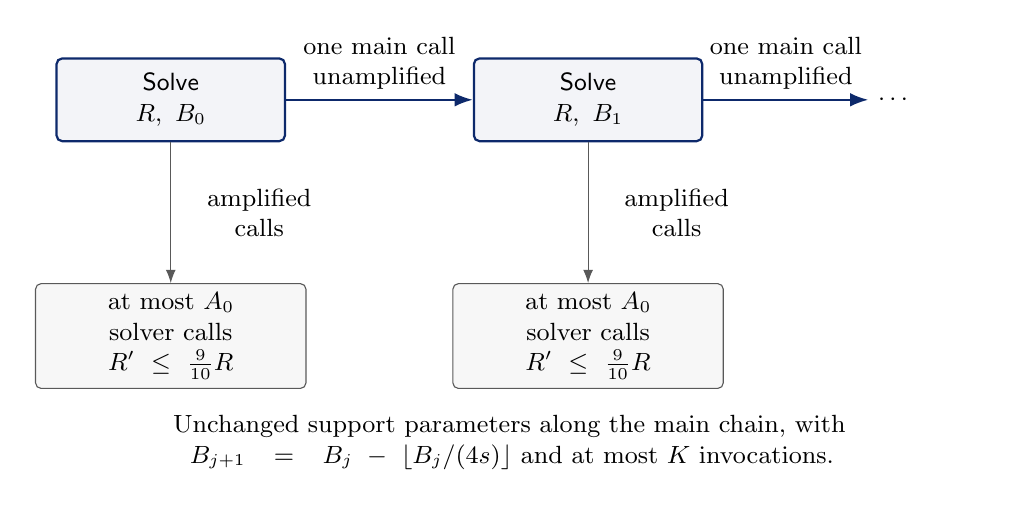
\begin{tikzpicture}[
  >=Latex,
  every node/.style={font=\small,align=center},
  main/.style={draw=linkblue,rounded corners=2pt,thick,
    fill=linkblue!5,minimum width=2.9cm,minimum height=1.05cm},
  reduced/.style={draw=black!65,rounded corners=2pt,
    fill=black!3,text width=3.2cm,minimum height=1.25cm},
  edge/.style={->,thick,draw=linkblue},
  side/.style={->,draw=black!65}
]
\node[main] (s0) at (0,0) {$\Solve$\\$R,\ B_0$};
\node[main] (s1) at (5.3,0) {$\Solve$\\$R,\ B_1$};
\node (dots) at (9.2,0) {$\cdots$};
\draw[edge] (s0) -- node[above,text width=2.3cm]
  {one main call\\unamplified} (s1);
\draw[edge] (s1) -- node[above,text width=2.3cm]
  {one main call\\unamplified} (dots);
\node[reduced] (r0) at (0,-3.0)
  {at most $A_0$ solver calls\\$R'\le\frac9{10}R$};
\node[reduced] (r1) at (5.3,-3.0)
  {at most $A_0$ solver calls\\$R'\le\frac9{10}R$};
\draw[side] (s0) -- node[right,text width=2.0cm]
  {amplified\\calls} (r0);
\draw[side] (s1) -- node[right,text width=2.0cm]
  {amplified\\calls} (r1);
\node[align=center,text width=12.0cm] at (4.3,-4.35)
  {Unchanged support parameters along the main chain, with
   $B_{j+1}=B_j-\lfloor B_j/(4s)\rfloor$ and at most $K$ invocations.};
\end{tikzpicture}
\caption{Contracting the main continuation chain. The lower boxes
represent all immediate smaller-rank $\Solve$ calls exposed inside
$\Ask$, $\Orient$, and $\OrientPlus$, including every trial and
repeated exceptional-set entry. The horizontal chain has only one
successor per nonterminal node and at most $K$ nodes, so it generates
at most $KA_0$ such descendants. These bounds hold on every random
tape. In the correctness proof, the same chain carries at most one
protected comparison until a local answer establishes it or the
terminal solver is reached.}
\label{fig:solver-recursion}
\end{figure}


Let \(N_d\) bound the total number of solver invocations generated
by one invocation of rank at most \(d\), including that invocation,
for the fixed graph and global parameters. A rank-zero invocation
returns directly. For positive rank, contract the main chain of at
most \(K\) invocations from Equation~\eqref{eq:main-chain-length}.
At each node of this chain there are at most \(A_0\) immediately
smaller-rank solver descendants. It follows that
\begin{equation}\label{cost:call-recurrence}
 N_0=1,\qquad N_d\le K+KA_0N_{d-1}\quad(d\ge1).
\end{equation}
There is only one main successor at each node, and its call is not
amplified. This is the reason one chain can be contracted. The
separation of one full-precision continuation from reduced-precision
calls also appears in Parys's parity-game recursion
\cite[Algorithm~2 and Section~5]{Parys2019}; here
Equation~\eqref{cost:branching} supplies the count for our particular
routines.

Equation~\eqref{cost:parameter-sizes} gives
\[
       K=O(x^2),\qquad A_0=O(x^{26}),\qquad KA_0=O(x^{28}).
\]
With \(A=KA_0\), induction in
Equation~\eqref{cost:call-recurrence} yields
\(N_d\le(K+1)(A+1)^d\). Since
\(D_*=O(\log x)\), we obtain
\begin{equation}\label{cost:call-count}
                N_{D_*}=2^{O((\log_2 x)^2)}.
\end{equation}
Every step of this count used a deterministic bound on every tape.
We must still bound the bit cost of the work done between these
solver calls.

\paragraph{Controlling integer magnitudes along an ancestry.}
The number of calls alone does not bound coordinate sizes, because
centered boxes can extend outside their parents. Consider any path
of ancestry in the full subroutine tree. Every child box is contained
in its parent except possibly a centered box
\[
        [q-A,q+A],\qquad A\in\{D,E_0\},
\]
formed by \(\Orient\). On every tape, its center \(q\) belongs to
the parent box, its radius satisfies \(A\le B/8\), and its reference
width is \(2A\le B/4\). All other transitions preserve or decrease
the reference width.

List the radii of just these centered transitions as
\(A_1,A_2,\ldots\). The first is at most \(B_*/8\). After a
transition of radius \(A_r\), the width is \(2A_r\) and cannot
increase before the next such transition. Therefore
\(A_{r+1}\le(2A_r)/8=A_r/4\). The possible outward displacement
of either endpoint is bounded by the convergent sum
\[
        \sum_{r\ge1}A_r
           \le\frac{B_*}{8}\sum_{r\ge0}4^{-r}
           =\frac{B_*}{6}.
\]
Starting from \([0,B_*]\), this proves that every actual endpoint,
center, and returned coordinate lies in
\begin{equation}\label{cost:endpoint-bound}
                       [-B_*/6,\,7B_*/6].
\end{equation}
These are real bounds on integer values; no rounding of the displayed
endpoints is intended.

The temporary sums used for midpoints, differences, scalar shifts,
and caps also have magnitude \(O(B_*)\). The operator \(F\) never
changes, and \(|t(e)|\le W\le B_*\), so each intermediate value
\(t(e)+p_j\) has the same order of magnitude. All such integers
therefore have \(O(\log_2(B_*+1))=O(x)\) bits. This includes
computations in centered boxes outside the original box, independently
of all comparison outcomes.

\paragraph{Representing the rational parameters exactly.}
Weights and budgets change only on a parameter-reducing edge into a
solver call. There are at most \(D_*\) such edges on any ancestry.
Starting from unit weights, every reachable coordinate weight is
\[
       \alpha_i=2^{-u_i^\alpha},\qquad \beta_i=2^{-u_i^\beta},
       \qquad u_i^\alpha,u_i^\beta\in\mathbb Z_{\ge0},\quad
       u_i^\alpha+u_i^\beta\le D_*.
\]
Starting from \(k=m=n\), the budgets have the forms
\begin{equation}\label{cost:budget-forms}
 k=n\frac{4^{u_k}3^{v_k}}{5^{u_k+v_k}},\qquad
 m=n\frac{4^{u_m}3^{v_m}}{5^{u_m+v_m}},\qquad
 u_k+v_k+u_m+v_m\le D_*,
\end{equation}
with nonnegative integer exponents. Hence each numerator and
denominator of a budget or weight has \(O(\log(n+1))\) bits.
One may store reduced fractions with binary integer numerators and
denominators, or store the exponents in these explicit forms.

Support sums admit a common power-of-two denominator of exponent at
most \(D_*\). The reciprocal-product sums used by \(R\) and
\(\mu\) are even simpler: for \(S\subseteq V\),
\[
       \sum_{i\in S}\frac1{\alpha_i\beta_i}
           =\sum_{i\in S}2^{u_i^\alpha+u_i^\beta}
           \le n2^{D_*}.
\]
Their bit lengths are \(O(\log(n+1))\). Exact integer arithmetic
thus computes these sums and tests \(R<1\) or \(\mu(S)>1/2\).
The support-budget tests and the height-threshold tests are likewise
exact after multiplication by positive denominators. Alternatively,
normalizing fractions with the Euclidean algorithm after each
operation gives polynomial bit cost without retaining a special
common-denominator representation.

The global integers \(g,s\) are computable by binary lengths and
integer comparisons with powers of two. Neither the rank nor the
real logarithms appearing in this proof must be evaluated by the
algorithm. The number \(2^{-J}\) is also solely an error bound;
no rational of that value is constructed.

\paragraph{Bounding the local work, including terminal iterations.}
The bit sizes are now controlled. For the small-width branch,
\(\Basic\) is used only when \(B\le128s\), and
Lemma~\ref{lem:box-solution} bounds it by
\[
                         1+128ns
\]
operator evaluations. Each evaluation scans the explicit edge list,
adding and comparing \(O(x)\)-bit integers, then clips the result.
This iteration count is independent of endpoint offsets and numerical
weight magnitudes. The other terminal branch, \(R<1\), uses no
iteration. Thus neither branch entails work proportional to \(W\)
or \(B_*\).

For a concrete representation, store a subset of \(V\) as an
\(n\)-bit incidence vector. Compute a coordinatewise median by
sorting the \(J\) entries in each coordinate and selecting entry
\((J+1)/2\). Majority votes, list concatenation, clipping, floored
averages, and coordinate extrema take polynomially many operations
on the bounded-size values above.

The work attached to one main-chain node includes at most
\(J(g+1)\) orientation invocations and polynomially many local
vector-loop steps. Terminal \(\Basic\) calls in these orientation
invocations contribute at most
\(J(g+1)(1+128ns)\) operator evaluations; they are not additional
solver invocations in \(N_d\). Keeping every center iterate and
every exceptional-list entry still uses polynomial local data and
work. Consequently the local work attached to one node, leaving its
solver calls unexpanded, is bounded by a polynomial \(P(L)\) of
absolute degree.

\paragraph{Generating bits and implementing the recursion.}
The only random primitive selects an iterate index. Because \(s\)
is a power of two, exactly \(\log_2s\) fair bits select a uniform
index from \(\{0,\ldots,s-1\}\), without a rejection loop. The
\(J\) trials in either amplification are run sequentially, taking
fresh bits from one tape. By Proposition~\ref{prop:termination},
each preceding subroutine terminates on every tape. Under fair
randomness the unread tail after this finite stopping time supplies
independent fresh bits, as required by the correctness proof. On a
fixed arbitrary tape the same execution respects every deterministic
call bound used above. Each orientation invocation reads at most
\(\log_2s\) bits of its own, already covered by its polynomial
local cost.

All routines are finite binary computations: \(\Ask\) performs its
\(J\) solver calls, and \(\OrientPlus\) performs its \(J\)
orientation calls. The final winning set requires \(n\) comparisons
with \(B_*/2\). Enlarge \(P\) to include this output step and the
preprocessing. For the total bit cost \(T_d\), contracting the main
chain as before gives
\begin{equation}\label{cost:bit-recurrence}
 T_0\le P(L),\qquad
 T_d\le KP(L)+KA_0T_{d-1}\quad(d\ge1).
\end{equation}
The estimates used in Equation~\eqref{cost:call-count} now yield
\(T_{D_*}=2^{O((\log_2(L+2))^2)}\).

A uniform machine can perform every instruction on binary strings.
Polynomial simulation overhead for data access or recursion in a
chosen standard model changes only the absolute constant in the
exponent. Arithmetic, storage manipulation, preprocessing, random
bits, and all recursive simulations are thereby included, on every
tape, in the asserted bound.
\end{proof}

\clearpage
\section{The complete algorithm and certified outputs}\label{sec:completion}

The preceding results now fit together without a further probabilistic
argument. One root call recovers the potential, and one threshold test
per vertex converts it to the required set.

\begin{proof}[Proof of Theorem~\ref{thm:main}]
From the explicit input compute $t,W,B_*$ according to
Equation~\eqref{eq:transformed}, and initialize the global parameters
of Equation~\eqref{eq:global-parameters}. Run
\[
 p=\Solve(0,B_*;B_*,\boldsymbol1,\boldsymbol1,n,n)
\]
and return $U_p=\{i\in V:p_i>B_*/2\}$. Scalars in the box positions
denote constant vectors.

Lemma~\ref{lem:box-solution} gives the unique deterministic solution
$x$ of $[0,B_*]$. Its two supports have size at most $n$ and so satisfy
the root budgets. By Corollary~\ref{cor:top-success}, the single event
$p=x$ has probability at least $7/8$. On that event,
Proposition~\ref{prop:game-reduction} identifies $U_p$ with the entire
zero-threshold winning set for the original weights and liminf payoff,
including against every opposing history-dependent strategy.

The computation terminates on every random tape by
Proposition~\ref{prop:termination}. Its full bit cost is bounded by
Theorem~\ref{thm:bit-complexity}, which already includes the
preprocessing and the $n$ final threshold comparisons. The procedures
use uniform finite instructions on binary integers, exact rationals,
and fair bits. Thus they supply both the stated output probability and
the asserted bound on every tape.
\end{proof}


The potential also provides a certificate that can be checked without
repeating the randomized proof. This gives a version that reports failure
instead of ever returning an incorrect answer.

\begin{corollary}[Certified winning regions and strategies]
\label{cor:certified-output}
There is a randomized algorithm which, on every tape, uses
$2^{O((\log_2(L+2))^2)}$ bit operations and returns either a failure
symbol or the exact winning set together with an integer potential and
positional strategies for both players. Whenever it returns these
objects, the Max strategy wins from every vertex of the winning set and
the Min strategy ensures upper limiting average at most $-1/n$ from
every other vertex, against arbitrary opposing strategies. It returns
these objects with probability at least $7/8$.

Repeating independent trials until a certificate is accepted terminates
almost surely, never returns an incorrect answer, and has expected bit
cost $2^{O((\log_2(L+2))^2)}$.
\end{corollary}

\begin{proof}
Run the root solver to obtain $p\in[0,B_*]$ and check
\[
                 p=\clip_{[0,B_*]}F(p).
\]
Accept precisely when this equality holds. By
Lemma~\ref{lem:box-solution}, it holds if and only if $p=x$, the
unique top-box solution. Thus acceptance certifies every coordinate,
and Corollary~\ref{cor:top-success} gives acceptance probability at
least $7/8$.

On acceptance, form $U=\{i:p_i>B_*/2\}$. At each Max vertex in
$U$, choose an outgoing edge attaining $F_i(p)$; at each Min vertex
outside $U$, choose an attaining edge as well. Complete the two
strategies arbitrarily at their other vertices. The two-band proof of
Proposition~\ref{prop:game-reduction} applies to the verified vector
$p=x$ and proves both strategy guarantees. The check and the edge
selections require a scan of the explicit edge list and arithmetic on
$O(L+1)$-bit integers, so they add only polynomial bit cost to the
bounded-time trial.

For independent repetitions, the probability that the first $r$ trials
all reject is at most $8^{-r}$. Hence acceptance occurs almost surely,
and the expected number of trials is at most
$\sum_{r\ge0}8^{-r}=8/7$. Multiplying by the worst-case bit cost of
one trial proves the expected-time bound. This repeated procedure has
no asserted time bound on every tape; each individual certifying trial
retains that bound.
\end{proof}

\appendix
\section{A counterexample to a tropical substitution rule}
\label{sec:tropical-comparison}

This appendix is independent of the game algorithm. It examines the
minimization variable-selection rule printed in Truffet's
\texttt{arXiv:2603.26423v4}, dated August~29, 2026
\cite{Truffet2026SubstitutionV4}. That version claims a strongly
polynomial tropical optimization algorithm and a mean-payoff consequence
through reductions. The example below loses its optimum under the stated
rule; the conclusion is confined to that version and procedure.

In ordinary arithmetic, consider
\begin{equation}\label{eq:substitution-example}
 \min x_1\quad\text{subject to}\quad
 \max(x_1,x_2)\ge0,\qquad x_1\ge\max(x_2+1,-2).
\end{equation}
The point $(0,-1)$ is feasible. Conversely, a feasible point with
$x_1<0$ would have $x_2\le x_1-1<0$, contradicting the first
constraint. Thus the true minimum is exactly zero.

\paragraph{Homogenization and the input conditions.}
The cited procedure homogenizes the constraint rows as
\[
 \max(x_1,x_2)\ge h,\qquad
 x_1\ge\max(x_2+1,h-2),
\]
and the objective as $z\ge x_1$; dehomogenization sets $h=0$.
Equation~(5b) of the cited paper holds for both ordered pairs of
constraint rows. Each left side lacks an $h$ term, whereas the other
row's right side has one. Setting $x_1=x_2=0$ and increasing $h$
therefore rules out the forbidden functional domination by any finite
additive constant. Both variables also have lower or upper occurrences, as required by
Definition~4.2 and Equation~(34). Choose the search endpoints
$\mu=0$ and $\lambda=-4$. They include the finite optimum witness
$(x_1,x_2,h)=(0,-1,0)$ and satisfy Equation~(23b) for the only
mixed lower function, $\max(x_2+1,h-2)$, since
\[
                 1+\lambda=-3<-2+\mu=-2.
\]
The lower function $h$ has no competing $x$ term.

\paragraph{The forced first selection.}
Numerotation convention~4.1 assigns index $0$ to the objective row.
The lower and upper occurrences in Equations~(24) and~(32) and
Definition~4.1 are drawn only from constraint rows $1,\ldots,m$.
For this instance they are
\[
 \begin{array}{c|c|c}
 \text{variable}&\text{lower-bound rows}&\text{upper-bound rows}\\\hline
 x_1&1,2&\varnothing\\
 x_2&1&2
 \end{array}
\]
In particular, the objective row is not an additional upper occurrence
of $x_1$. The lower branch for $x_2$ is $x_2\ge h$ in row~1; its
upper bound is $x_2\le x_1-1$ in row~2. Equation~(53a) therefore
makes the dominating-variable set exactly $\{x_2\}$. Equation~(53b)
restricts eligible lower inequalities to that set, leaving the unique
pair $(1,2)$. Theorem~4.3, Equation~(47), and Section~4.2.3,
Case~2.2.2, prescribe saturation of this selected inequality:
\[
 x_2=h.
\]
There is no tie-breaking choice in this step.

\paragraph{The resulting loss of the optimum.}
After substitution the second row requires $x_1\ge h+1$. The next
eligible saturation consequently sets $x_1=h+1$. The stopping test in
Equation~(39) fails before each of these two substitutions. At both
stages the objective still depends on $x_1$, so the separate rule for
an objective-independent switch to maximization does not apply.
Normalizing to $h=0$ gives objective value $1$, whereas the original
minimum in Equation~\eqref{eq:substitution-example} is $0$.

The first substitution already removes every optimum: selecting a
lower-bound disjunct on the basis of an upper occurrence of its variable
does not preserve the optimum of these coupled constraints. This
calculation does not address a different variable-selection rule, a
repaired algorithm, or another version. In particular, it is not an
assessment of the distinct 2025 HAL/MSR max-atom proof discussed in the
introduction. None of the results of that work or of the cited tropical
procedure is used in the proof of Theorem~\ref{thm:main}.

\bibliographystyle{plain}
\bibliography{references}
\end{document}
